\chapter{Evaluation and results}
\label{chap:eval}

In the previous chapter, the evaluation suite and its features were presented.
This chapter is split into several sections.
First, it deals with the introduction of datasets, so which datasets were evaluated and why.
Second, the quality metrics for the comparison of disparity algorithms for stereoscopic videos are defined.
Third, the structure of the measurement is illustrated.
How the measurement were processed and visualized.
Fourth, the results are presented and discussed.
\newline\newline\noindent Overall, the setup for the evaluation took more than 28 days to process about 50 GB of stereoscopic videos and to create all disparity maps.
Accumulated, the computed disparity maps, the created masks as well as the heatmaps, allocated about 18 GB.

\section{Datasets}

A dataset basically describes a set of stereo images, which additionally contains ground-truth disparity maps.
The aim of such datasets is to provide accurate data, on which researchers can rely.
This datasets can be used to evaluate the performance of computer vision algorithms, such as disparity algorithms in this thesis.
Without having such datasets it would be crucial to rate the overall quality of for instance stereo matching algorithms.
As for today, no high-resolution stereoscopic video dataset yet exists, neither a synthetic nor a captured one.
In order to obtain ground-truth depth information, there exist in general two options.
On the one hand, the real-world can be sensed via area scanner, for instance a radar (cf. KITTI vision benchmark suite\footnote{\url{http://www.cvlibs.net/datasets/kitti/}}).
On the other hand, a synthetic computer-animated scene is generated and the renderer calculates the disparity.
Of course, the former approach is more error-prone than the latter one.
The former one can lack of accuracy due to false measurements whereas the latter one real ground-truth information provides.
\newline\newline\noindent \citeauthor{kondermann2015stereo} came up with an interesting approach.
As area scanners are never 100 percent accurate, they introduced error-bars, which can range from $0-10$.
An error-bar indicates how certain the area scanner was that this disparity for a given pixel really existed \citep{kondermann2015stereo}.
As it would be a tremendous task to evaluate every existing stereoscopic dataset with every existing disparity algorithms, here three different datasets were chosen.
Other datasets, which were found but not investigated are the MPI Sintel Stereo Training Data, created for optical flow evaluation \citep{Butler:ECCV:2012} and the Middlebury stereo dataset, providing real images with ground-truth information \citep{scharstein2006middlebury}.

\subsection*{Tsukuba stereo dataset}

As reference dataset, the reworked Tsukuba Stereo Dataset was chosen \citep{martull2012realistic}.
One of the three scenes is called tsukuba to honour the popular \textit{Head and Lamp} scene and was shortly introduced in the foundations Chapter \ref{chap:foundations}.
The reference dataset is used to see if the implementation leads to similar results as in other stereo benchmarks.
This does of course not verify that the presented implementation is error-free but can point in the right direction.
Of course, the settings (i.e. parameters of an algorithm) depends on the input material (e.g. size of the images, noise occurrences) and on the type of the scenery, for instance many regions with arbitrary surfaces (textured vs textureless).
Hence, it is possible to have good parameters for one scene and not for the other.
However, in order to evaluate those algorithms the reference dataset is used to see how the eval engine actually works with the same parameters on the same images.

\begin{figure}[h!]
\centering
\begin{tabular}{ccc}
\subfloat[tsukuba scene]{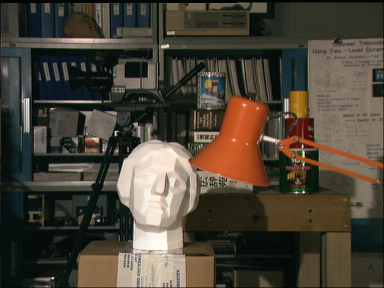
\includegraphics[width=0.3\textwidth]{src/images/tsukuba-imgL.png}} &
\subfloat[teddy scene]{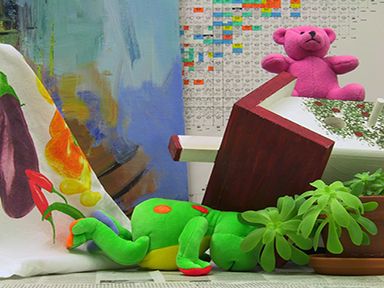
\includegraphics[width=0.3\textwidth]{src/images/teddy-imgL.png}} &
\subfloat[venus scene]{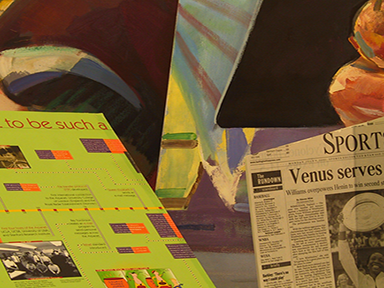
\includegraphics[width=0.3\textwidth]{src/images/venus-imgL.png}} \\
\subfloat[tsukuba disparity]{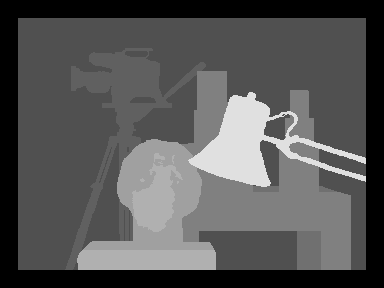
\includegraphics[width=0.3\textwidth]{src/images/tsukuba-dgt.png}} &
\subfloat[teddy disparity]{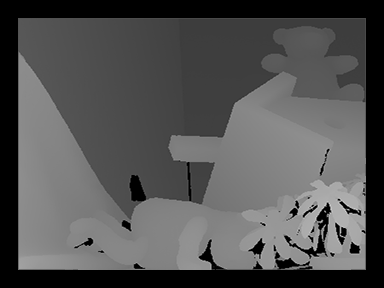
\includegraphics[width=0.3\textwidth]{src/images/teddy-dgt.png}} &
\subfloat[venus disparity]{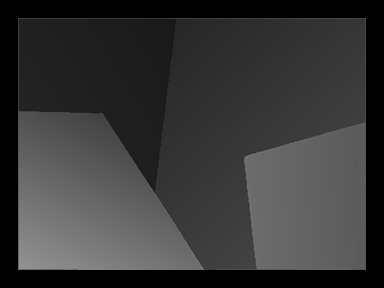
\includegraphics[width=0.3\textwidth]{src/images/venus-dgt.png}} \\
\end{tabular}
\caption[Tsukuba stereo dataset]{Tsukuba stereo dataset \citep{martull2012realistic}}
\label{fig:tsukuba2}
\end{figure}

\subsection*{Cambridge stereo dataset}

The second one is a dataset, especially created for the evaluation of the DCBGrid from the University of Cambridge\footnote{\url{http://www.cl.cam.ac.uk/research/rainbow/projects/dcbgrid/datasets/}}.
This is also one of the first stereoscopic dataset targeting videos.

\begin{figure}[h!]
  \centering
  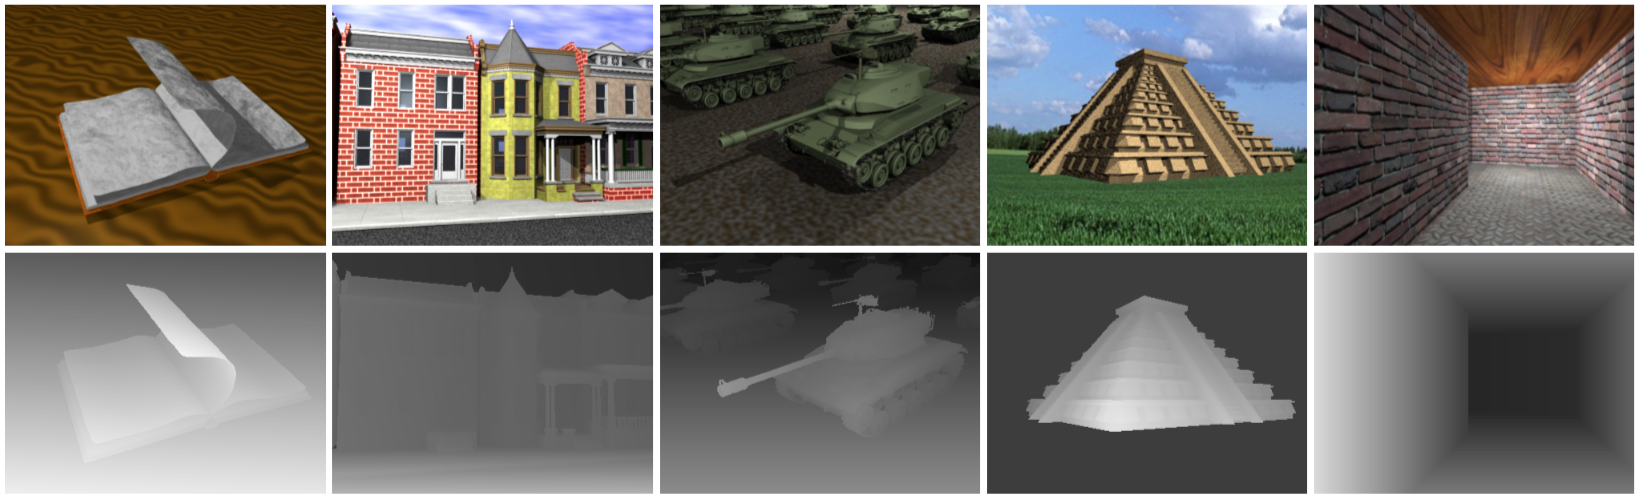
\includegraphics[width=1.0\textwidth]{src/images/dbcgrid-dataset.png}
  \caption[Cambridge stereo dataset example]{Cambridge stereo dataset example}
  \label{fig:dbcgrid-dataset}
\end{figure}

\noindent The Cambridge stereo dataset consists of five different rendered scenes in $400x300$ resolution with each about 100 frames \citep{richardt2010real}.
The dataset scales the disparity for each scene from $0$ to $64$.
The disparity maps are delivered as PNG image files, ranging from $0-255$.
Thus, the disparity maps are loaded into a matrix and simply converted to range from $0-64$ by dividing the whole matrix through $4$.
Beforehand, the matrix is converted into $CV_32F$, meaning that each element is represented by 32-bit floating values.

\subsection*{SVDDD - a high-resolution Stereoscopic Video Dataset with precise Depth and Disparity information}

As third dataset, a novel, not yet analyzed dataset was chosen: the SVDDD\footnote{SVDDD stands for a high-resolution Stereoscopic Video Dataset with precise Depth and Disparity information.} dataset.
The department of Praktische Informatik IV\footnote{\url{http://ls.fmi.uni-mannheim.de/de/pi4/}} created the dataset on its own with high-resolution video sequences containing accurate depth and disparity information for stereoscopic videos.
Figure \ref{fig:eval:svddd:intro} depicts the left image and its ground-truth disparity companion for a small selection of the SVDDD dataset.
\newline\newline\noindent The difference here is, that this dataset was not analyzed before.
Thus, it is possible that the chosen algorithms work not properly on this dataset.
If this case occurs there exist two possibilities why this happens.
On the one hand, the disparity information are not properly calculated, or on the other hand, those algorithms have some troubles with the constructed scenery.

\begin{figure}[h!]
\centering
\begin{tabular}{cc}
\subfloat[02-rabbit, left image]{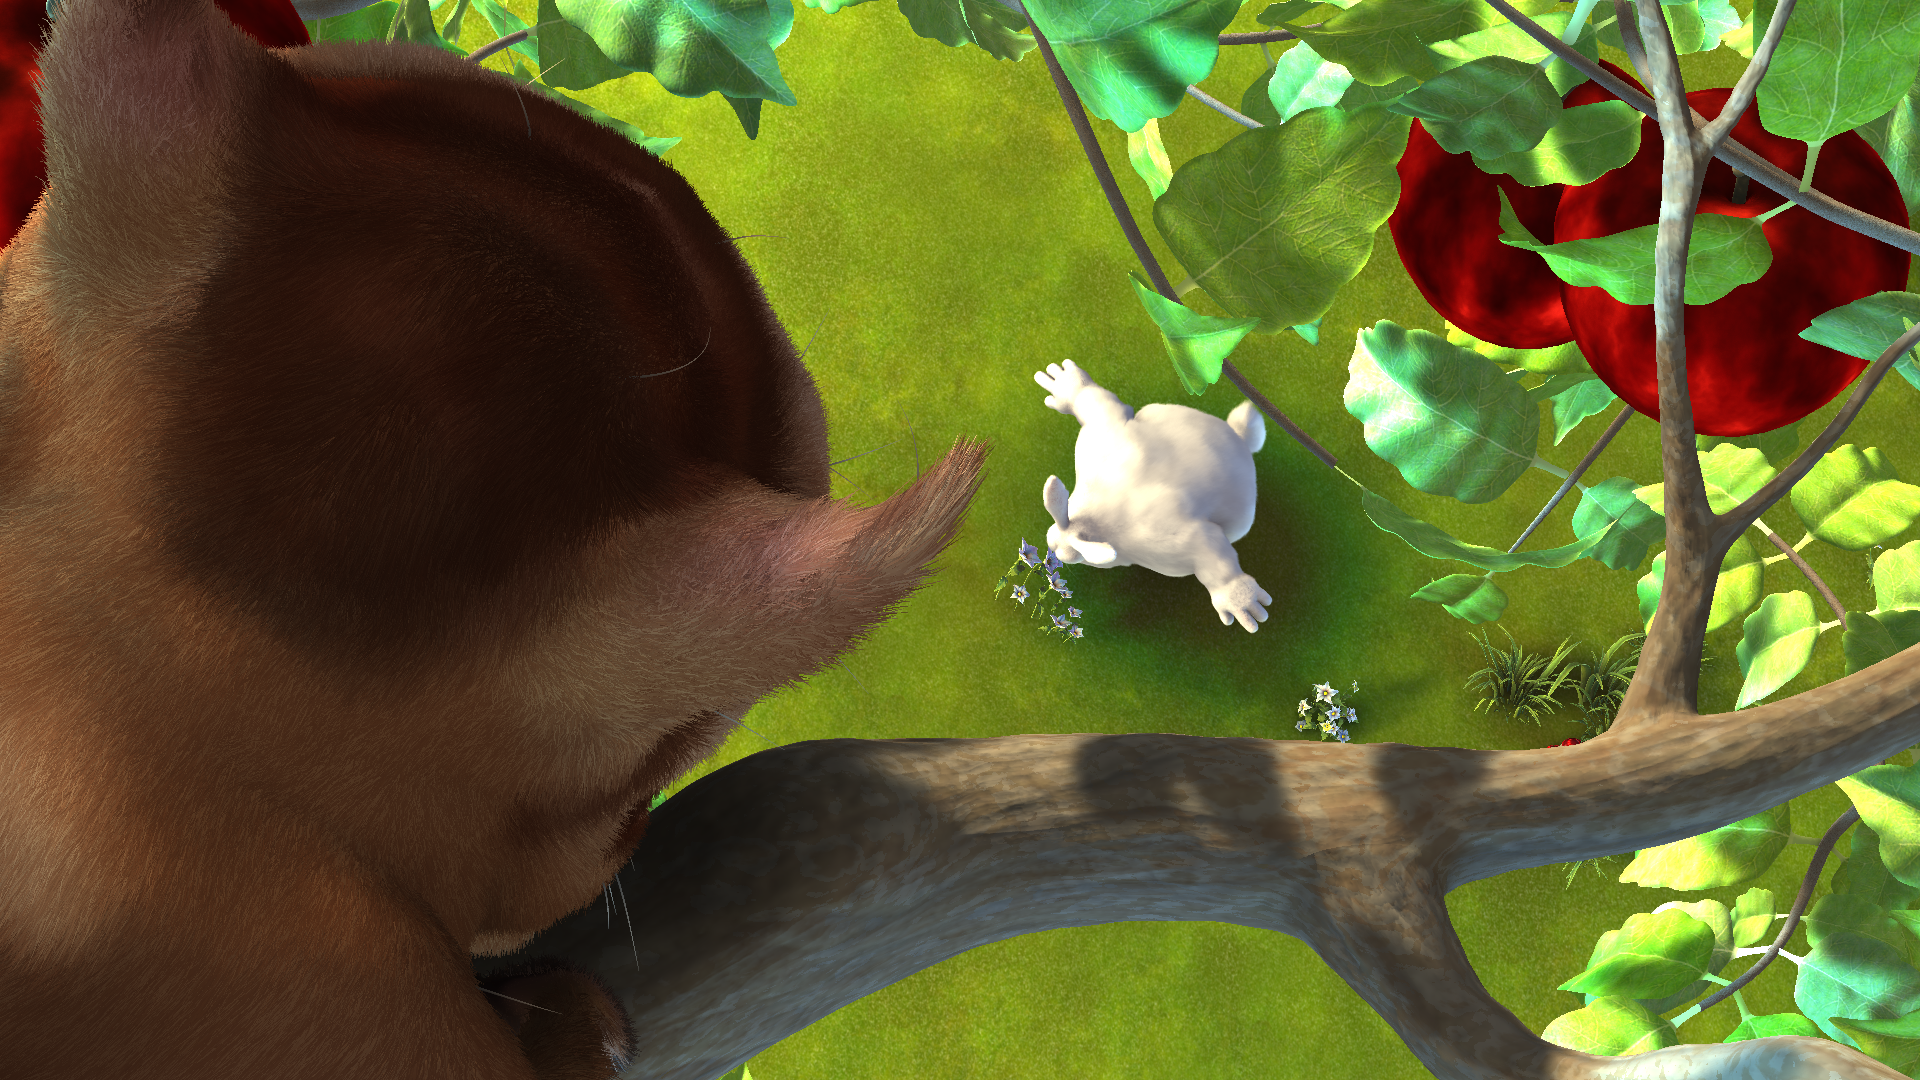
\includegraphics[width=0.45\textwidth]{src/images/evaluation/svddd/02-rabbit-left.png}} &
\subfloat[03-apple, left image]{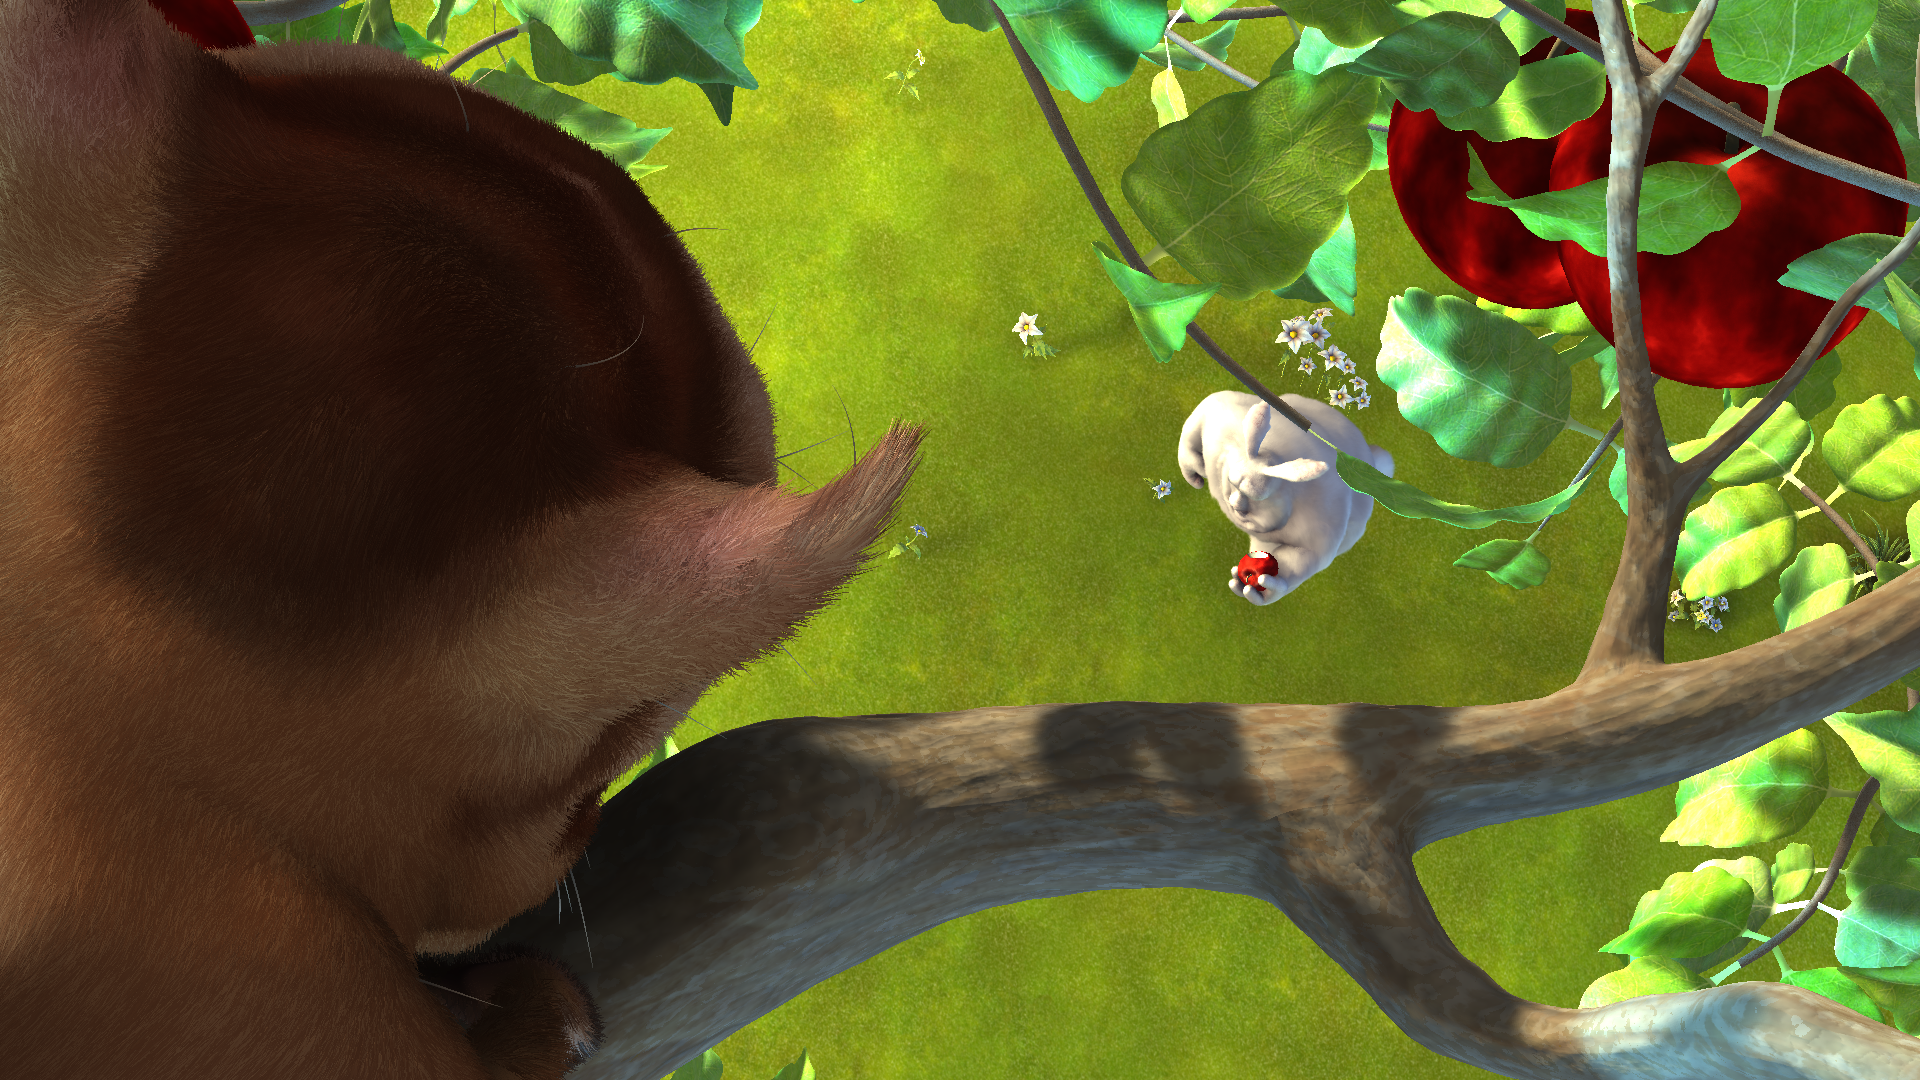
\includegraphics[width=0.45\textwidth]{src/images/evaluation/svddd/03-apple-left.png}} \\
\subfloat[02-rabbit, disparity]{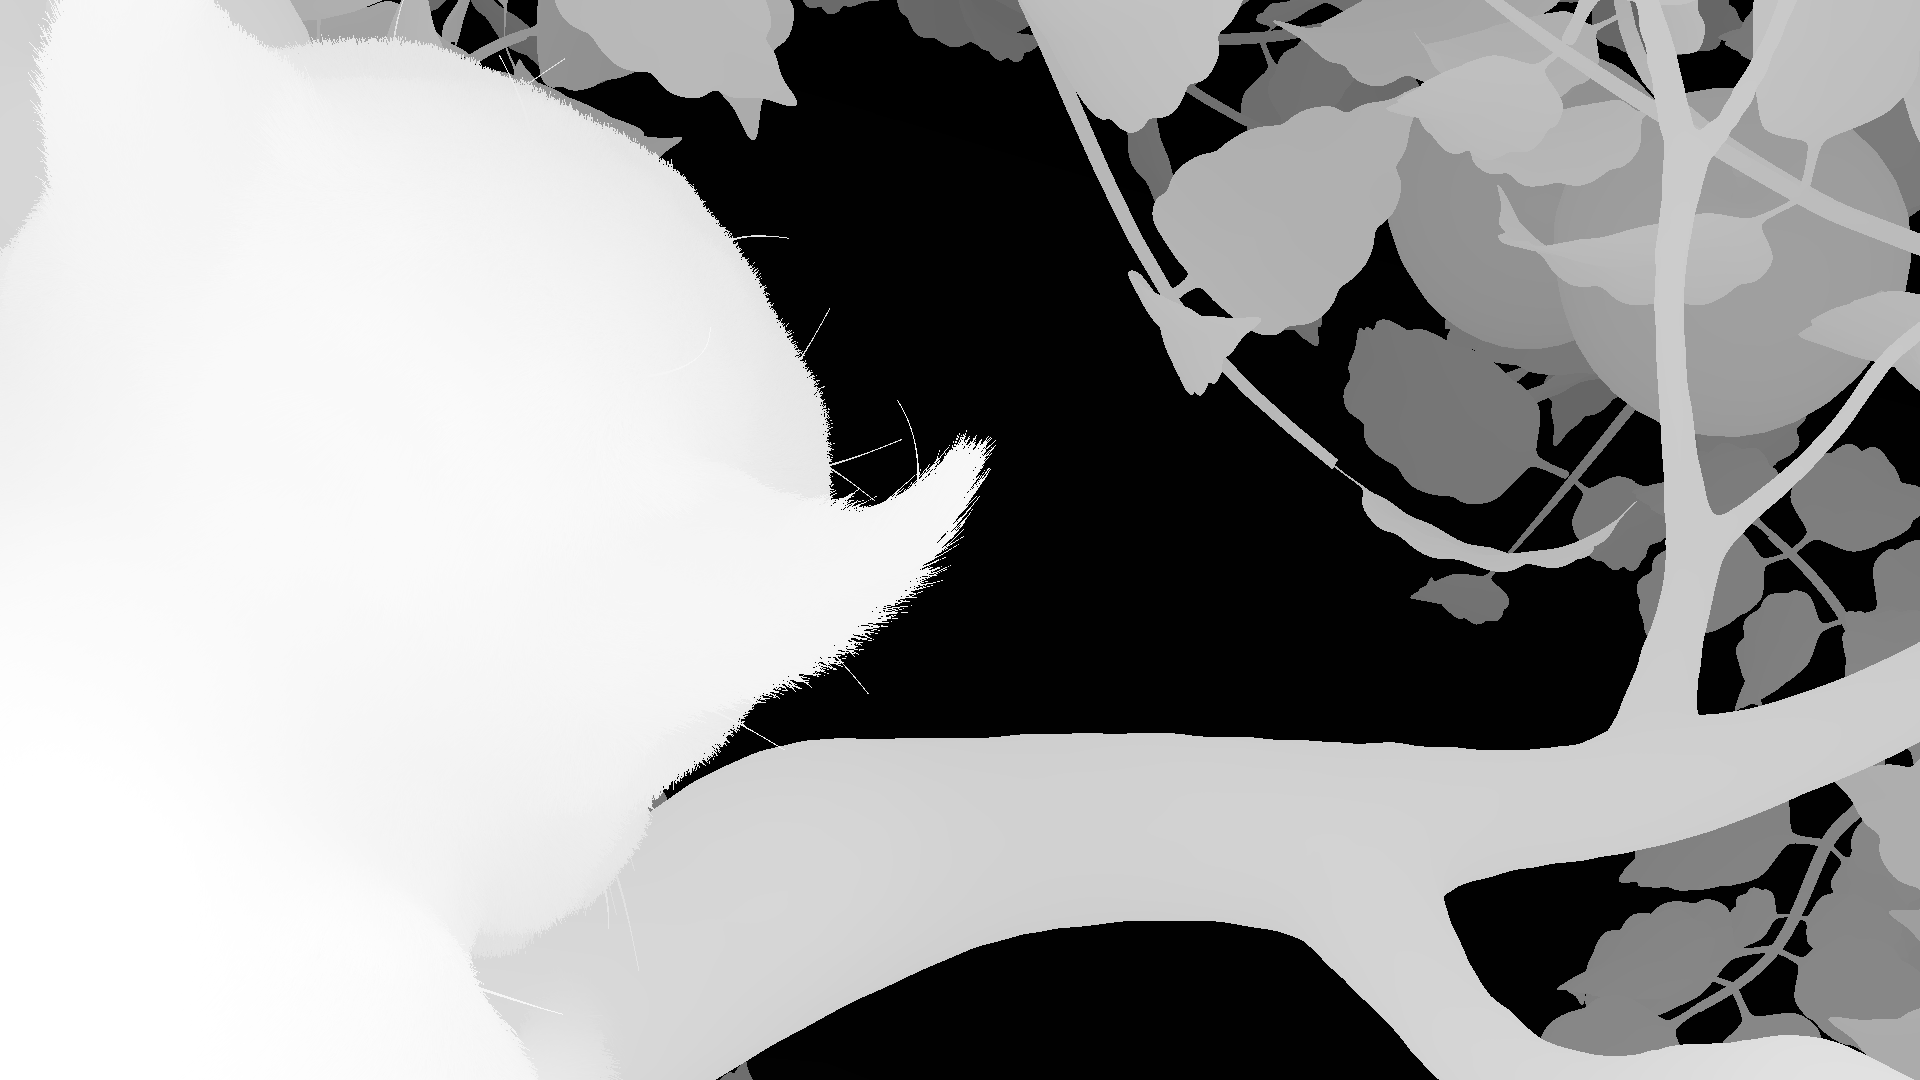
\includegraphics[width=0.45\textwidth]{src/images/evaluation/svddd/02-rabbit-disparity.png}} &
\subfloat[03-rabbit, disparity]{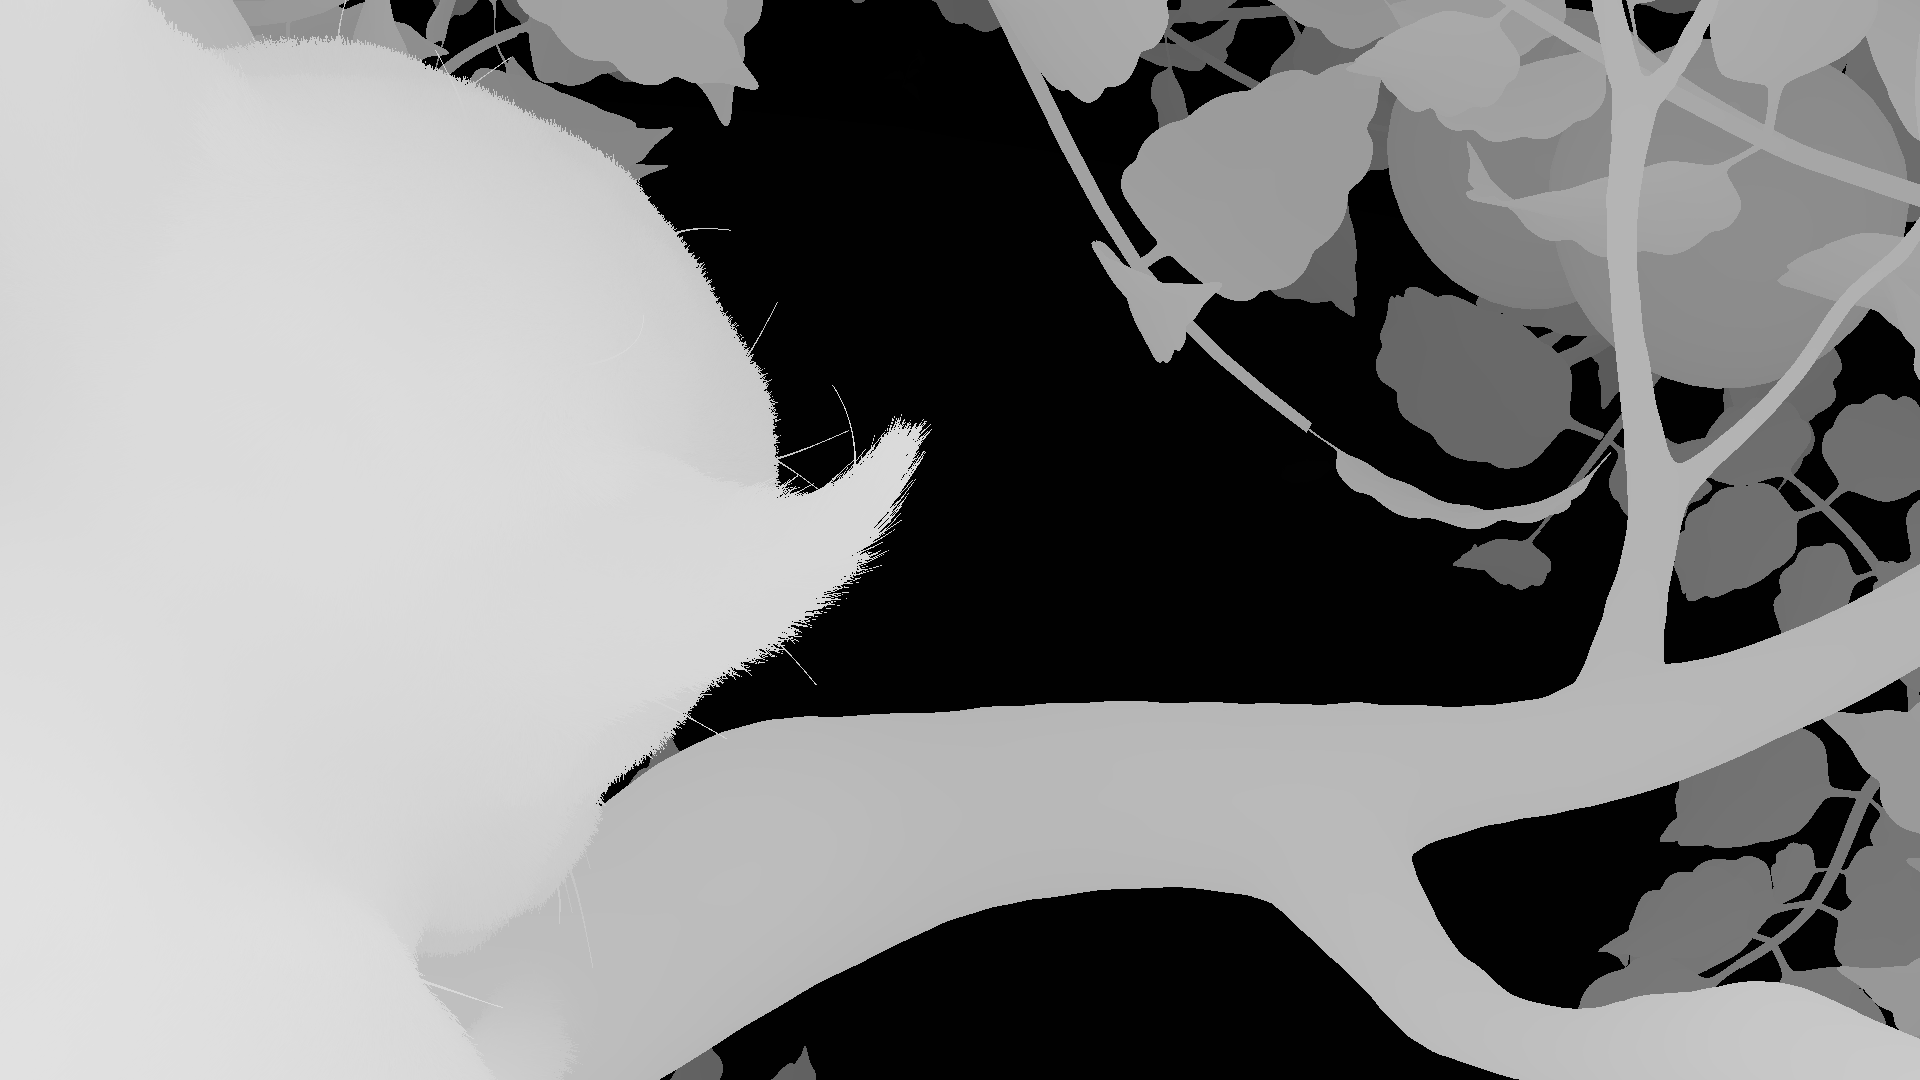
\includegraphics[width=0.45\textwidth]{src/images/evaluation/svddd/03-apple-disparity.png}}
\end{tabular}
\caption{SVDDD high-resolution stereo dataset}
\label{fig:eval:svddd:intro}
\end{figure}

\noindent Focusing on the latter one, the scenes were created with Blender and utilizes open-source scenes from the Big Buck Bunny project\footnote{\url{https://peach.blender.org}}.
A second camera was added to the scenes for obtaining depth information.
The parameter for each scene can be extracted from the Blender files.
The scenes were also adjusted regarding the following points to extract depth-information accurately.
Rays of light as well as transparent layers were removed to retain accurate depth-information.
Such transparent layers may result in anomalous depth-information as they may bounce back the depth request while obtaining depth information from Blender.
Those transparent layers are in between the actual background of the scene, which is visible for the viewer, and the camera.
Motion and object blur were reduced as such areas can yield to defective disparity information around the blur.
Fain-grained textures like grass or fine hairs were modified.
Without modifying these elements in a scene, a stereo matching algorithm may have problems with those arbitrary textures.
The initial scenes of the Big Buck Bunny project contained randomized grass in each image, left and right side.
This also yields in the impossibility of stereo matching algorithms to determine the shift of the pixels.
\newline\newline\noindent The dataset consists of 15 scenes.
The scenes consist of high resolution stereo images $1920x1080$ with an average bitrate of 94 MBit/s.
With an approximate size of 2 MB for each frame, the size of each sequence varies between 0.4 GB and 2.7 GB.
For each frame, depth and disparity information are computed with 32-bit floating point precision and saved in OpenEXR files.
The above mentioned points apply to the first alpha version of the dataset.
During this thesis, the dataset ran through several iterations as more and more problems arose during the evaluation.
This is discussed later on.

\section{Quality metrics}

Typical quality measure instruments for comparing disparity maps against their ground-truth reference data are  \citep{cyganek2011introduction}:

\begin{itemize}
  \item percentage of bad matching pixels,
  \item root-mean-square error,
  \item parameter-free measures.
\end{itemize}

\noindent As parameter-free measures needs modified disparity algorithms \citep{cyganek2011introduction}, it was not considered.

\subsection*{Percentage of bad matching pixels}

Percentage of bad matching pixels (PBMP) is usually used in comparing the performance of stereo matching algorithms.

\begin{equation}
  \operatorname{PBMP}=\frac{1}{n} \sum_{x,y=0}^{}(|d_a(x,y) - d_e(x,y)| > \delta_t)
\end{equation}

\noindent The threshold, denoted with $\delta_t$, can be adjusted and as result, the percentage of outlier pixels, which differ by more than $\delta_t$, is estimated.

\subsection*{Root-mean-squared error}

The mean squared error (MSE) as well as the root mean squared error (RMSE) are both the most popular metrics in image and video processing \citep{cyganek2011introduction, benoit2008quality, scharstein2002taxonomy}.
The MSE is, as the name implies, the mean of the squared differences between the intensities of pixels in two pictures at the same position.
In conclusion, the average difference per pixel is then the root of the squared error.

\begin{equation}
  \operatorname{RMS-Error}=\sqrt{\frac{1}{n} \sum_{x,y=0}^{}(d_a(x,y) - d_e(x,y))^2}
\end{equation}

\noindent It represents the sample standard deviation of the differences between predicted values and observed values.
Here $d_a(x,y)$ is the actual disparity value for given $x$ and $y$.
$d_e(x,y)$ is our expected disparity value from our ground-truth data.
Hence the RMSE is the difference between values on average.

\section{Measurement}

This chapter summarizes the thoughts behind the evaluation.
All disparity maps were created on a desktop computer with an i5-2500k @ 3.30GHz (quad-core).
First, the idea of a distributed calculation arose, as described in Chapter \ref{chap:impl}.
As this would lack the comparison of runtime, only the desktop computer was used.
\newline\newline\noindent The whole evaluation was proceeded like the following:
Python scripts for the execution of all components in a chain were written.
Disparity maps are computed for each frame in a sequence, for each sequence in a dataset, and for each dataset.
The Cambridge dataset contains five sequences with each 100 frames.
In total 12 algorithms were executed.
This makes an amount of $6.000$ disparity maps.
\newline\newline\noindent In addition, this dataset was duplicated for observing interferences on disparity algorithms.
For analyzing the impact of noise, additive gaussian noise with a normal distribution of $\mathcal{N}(\mu,\sigma^2)$ was added.
For $\sigma$, $10, 20, 30$ were chosen as parameter.
Lower values had no real impact on a few sample disparity maps computations and were also not visually exhibited.
Higher values were analyzed by \citeauthor{richardt2010real} \citep{richardt2010real}, but are clearly disturbing the whole image.
As additive gaussian noise should simulate a more real scenery instead of synthetic rendered videos, higher values were not considered.
\newline\newline\noindent Normally, high resolution videos are not transmitted in their pure nature (lossless), for instance raw files.
That said, H.265 was chosen as current state of the art video compression codec.
H.265 was introduced in Chapter \ref{chap:impl}.
For analyzing the disturbing effects on disparity algorithms, video compression artifacts were added by converting the images to a video, applying the codec and unwrapping the video into images.
As parameter, the constant rate factor (CRF) can be adjusted.
The default parameter value is $28$.
As $0$ means lossless video compression, it was tested with a few sample disparity maps computations.
$0$ had no impact and was not considered for the evaluation.
$51$ was not considered as well, as this totally disturbs the image visually, even if there is no motion between two consecutive frames.
$14, 28, 40$ were chosen as final values to have a feasible amount of different values and also a meaningful jump between those values (always half steps).
\newline\newline\noindent Taking those combinations into account yields to an amount of disparity maps to be computed of $48.000$.
After the disparity maps were computed, other Python scripts were written and executed for the aggregation of the results.
As the results are for each image in a sequence from a dataset and also focusing on one algorithm, they have to be aggregated and written in summarized CSV files.
The simple stereo matcher was treated as an exception.
The reason for this is simple: all the scripts were written with the intent of calculating single independent disparity maps.
As the simple stereo matcher features spatiotemporal consistency, scripts focusing especially on the execution and aggregation of this matcher were written as well.

\subsection*{Parameter tuning}

The observed parameters regarding noise and video compression were described before.
In addition, most of the available parameters were described accurately in Chapter \ref{chap:impl}.
Adjusting and quantifying also the parameters of each algorithm would be a formidable task.
Thus, only the maximum disparity was adjusted according to the dataset.
All the other variables were left as default and moreover, some algorithms have no parameter but the maximum disparity to adjust.

\subsection*{Visualization}

As it may be hard to identify fine-grained changes in grayscale images and also the human eye tends to be more sensitive to observe color changes, heatmaps are used to visualize the results.
For visualization, the heatmaps are created with the OpenCV autumn color scheme.
The color-scale of this theme is depict in Figure \ref{fig:colorscale}.

\begin{figure}[h!]
  \centering
  
\includegraphics[width=0.6\textwidth]{src/images/colorscale.png}
  \caption[OpenCV autumn color scale]{OpenCV autumn color scale\protect\footnotemark}
  \label{fig:colorscale}
\end{figure}
\footnotetext{Source (accessed 04/2016): \url{http://docs.opencv.org/3.1.0/d3/d50/group__imgproc__colormap.html}.}

\noindent Outliers are marked with three different purple color steps in the heatmaps.
The darker the purple color is, the more hard the error was.
The light blue means $1px$ threshold was exceeded, the color in-between the light blue and the dark purple denotes $2px$ threshold was exceeded and the very dark purple reflects $4px$ threshold was exceeded.
The border is excluded from the evaluation (cf. Chapter \ref{chap:foundations}) and marked black.
Brighter color means more heat and marks nearer pixels.
An example shot can be seen in Figure \ref{fig:example-heatmap}.
\newline\newline\noindent The maximum disparity in this example shot was $64$.
This means that due to the baseline separation of the cameras, and the resulting shift of the pixels, some pixels can not be calculated as they have no counterpart.
This was excluded from the evaluation.
Also, as the area-based disparity algorithms work with a window size and have a small step from the top and the bottom, this was excluded as well.
Both is represented with a border mask, which was applied to all evaluation steps beforehand.
This can also be seen in Figure \ref{fig:example-heatmap}.
This guarantees a streamlined and balanced evaluation.

\begin{figure}[h!]
\centering
\begin{tabular}{cc}
\subfloat[outliers heatmap]{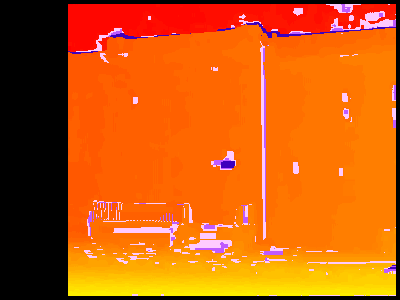
\includegraphics[width=0.45\textwidth]{src/images/evaluation/street-example-heatmap-outliers.png}} &
\subfloat[ground-truth heatmap]{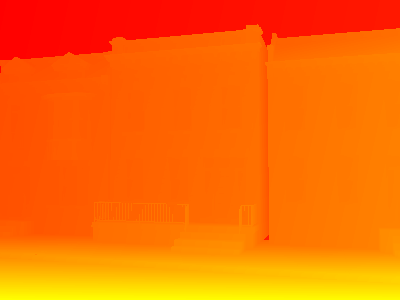
\includegraphics[width=0.45\textwidth]{src/images/evaluation/street-example-heatmap.png}}
\end{tabular}
\caption[Example heatmaps]{Example heatmaps for outliers heatmap and disparity ground-truth.}
\label{fig:example-heatmap}
\end{figure}

\subsection*{Applying disparity algorithms on videos}

As said in the implementation Chapter \ref{chap:impl}, disparity algorithms for image can be applied to videos.
Although the frames of a video can be seen as independent pieces, different anomalies can be further investigated while analyzing videos:

\begin{itemize}
  \item outliers in the form of a single frames which differs too much from the others,
  \item impact of additive Gaussian noise to simulate real scenery,
  \item impact of disturbing effects like artifacts from video compression,
  \item the benefit from creating a naive spatiotemporal context.
\end{itemize}

\noindent The following sections present only the highlights of the results as it is an tremendous amount of data, which were computed during the evaluation.

\section{Results}

The highlights are illustrated as the amount of information, which were obtained during the measurement is huge.
The following Table \ref{tab:identifier1} contains the identifier which are used throughout the upcoming subsections.
Algorithm (10) OpenCV - simple BM utilizes the same implementation as (2) OpenCV - BM but without performing a left-to-right consistency check and WLS filtering, as described in Chapter \ref{chap:impl}.
The following subsections are rationed in the results against the reference dataset, the general performance of the Cambridge dataset as well as the impact of interferences like noise and video compression.
Afterwards, the runtime and the SVDDD dataset are outlined.
As of now, the spatiotemporal approach with unweighted matching cost is denoted as \textit{SNSM - STU} whereas the weighted spatiotemporal approach is denoted as \textit{SNSM - STW}.

\begin{table}[h!]
\centering
\begin{tabular}{ll}
  \hline
  \textbf{Id} & \textbf{Sequence} \\ \hline \hline
  1 & book \\
  2 & street \\
  3 & tank \\
  4 & temple \\
  5 & tunnel \\
  & \\
  & \\
  & \\
  & \\
  & \\
  & \\
  & \\
  & \\
  \hline
\end{tabular}
\quad
\begin{tabular}{ll}
  \hline
  \textbf{Id} & \textbf{Algorithm} \\ \hline \hline
  1 & OpenCV - SGBM \\
  2 & OpenCV - BM \\
  3 & ELAS \\
  4 & MRF - ICM \\
  5 & MRF - GC Expansion \\
  6 & MRF - GC Swap \\
  7 & MRF - BP TRWS \\
  8 & MRF - BP BPS \\
  9 & MRF - BP BPM \\
  10 & OpenCV - Simple BM \\
  11 & SNSM \\
  12 & SNSM - STU \\
  13 & SNSM - STW \\
  \hline
\end{tabular}
\footnotetext{Simple stereo matcher with respecting spatiotemporal context, unweighted.}
\footnotetext{Simple stereo matcher with respecting spatiotemporal context, weighted.}
\caption{Identifier for results}
\label{tab:identifier1}
\end{table}

\noindent The general procedure is to describe the high level results of algorithms operate on a whole sequence with PBMP$_{1px}$ utilizing the non-occluded mask.
As the focus is on PBMP$_{1px}$, lower results are better.
The cell of the best result in each row is marked with green background color, the worst with red.
Then, the other masks are outlined in greater detail.
Afterwards, particular outliers regarding the whole sequence are discussed.
The same procedure is then applied to impact of noise and impact of video compression.

\subsection{Against reference dataset}

As reference scene the \textit{Head and lamp} scene of the Tsukuba dataset was chosen.
For evaluating against the reference dataset, all presented disparity algorithms computed disparity maps.
These disparity maps are then compared in combination with different masks.
The result can be seen in Table \ref{tab:eval:snsm:tsukuba} and the SNSM is depicted in Figure \ref{fig:eval:snsm:tsukuba}.
Compared with the Middlebury stereo benchmark\footnote{\url{http://vision.middlebury.edu/stereo/eval/}}, similar results could be achieved.
\newline\newline\noindent The SNSM utilizes SAD as matching cost function and does not further disparity refinement.
The results from SNSM with a threshold of $1$ and a block size of $9$ are PBMP$_{all,1px}$ = 11.51\% and RMSE$_{all} = 1.78px$.
According to the Middlebury stereo benchmark, the other SAD implementation (SAD-IGMCT) \citep{ambrosch2010accurate} achieved with a threshold of $1$: PBMP$_{all,1px}$ = 7.14\%.
The difference may come from smoothing, which SAD-IGMCT included as a disparity refinement step, which is visible while looking at their outcome.
The other results are similar to the results in the Middlebury stereo benchmark.
Some deviations like SAD-IGMCT to SNSM regarding all pixels and a threshold of $2$ are huge but can be explained with disparity refinement steps which the SNSM does not perform.

\begin{table}[h!]
\centering
\scalebox{0.95}{
\begin{tabular}{l|rrrr}
  & RMSE$_{all}$ & PBMP$_{all,1px}$ & PBMP$_{all,2px}$ & PBMP$_{disc,2px}$ \\ \hline
(1) OpenCV - SGBM & 1.49px & 7.00\% & 4.73\% & \cellcolor{green!50}11.99\% \\
(2) OpenCV - BM & 1.45px & 10.27\% & 5.92\% & 12.40\% \\
(3) ELAS & \cellcolor{green!50}1.23px & 7.07\% & \cellcolor{green!50}4.42\% & 12.08\% \\
(4) MRF - ICM & 5.02px & 22.32\% & 18.83\% & 19.72\% \\
(5) MRF - GC Expansion & 2.56px & 5.59\% & 4.74\% & 12.86\% \\
(6) MRF - GC Swap & 2.79px & 5.55\% & 4.70\% & 12.74\% \\
(7) MRF - BP TRWS & 2.48px & 5.41\% & 4.54\% & 12.32\% \\
(8) MRF - BP BPS & 2.64px & 9.49\% & 9.07\% & 16.27\% \\
(9) MRF - BP BPM & 2.55px & \cellcolor{green!50}5.34\% & 4.97\% & 12.99\% \\
(10) OpenCV - Simple BM & \cellcolor{red!50}6.10px & \cellcolor{red!50}28.27\% & \cellcolor{red!50}26.42\% & \cellcolor{red!50}28.99\% \\
(11) SNSM & 1.78px & 11.51\% & 9.85\% & 18.97\% \\
SAD-IGMCT & - & 7.14\% & 5.80\% & 18.90\% \\ \hline
\end{tabular}
}
\caption[Result table for reference dataset]{Result table for reference dataset}
\label{tab:eval:snsm:tsukuba}
\end{table}

\noindent The best result is achieved with a variant of a global method, belief propagation and yields to 4.97\% of bad matching pixels regarding all pixels and applying a threshold of $2$.
ELAS performs pretty good but struggles with a very accurate disparity map while comparing the results for PBMP$_{all,1px}$.
The simple block matching algorithm of OpenCV (10) is the same as (2), but without the disparity refinement step and a left-right-consistency check.
This may explains the very bad results.
Surprisingly, the global methods do not outperform the local methods by far.

\begin{figure}[h!]
\centering
\begin{tabular}{cc}
\subfloat[ground-truth heatmap]{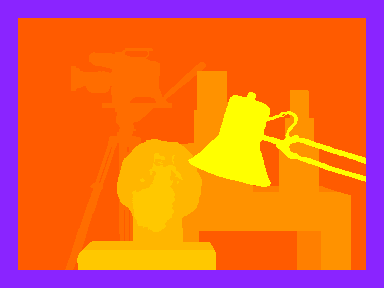
\includegraphics[width=0.45\textwidth]{src/images/evaluation/snsm-tsukuba-ground-truth.png}} &
\subfloat[computed disparity-map]{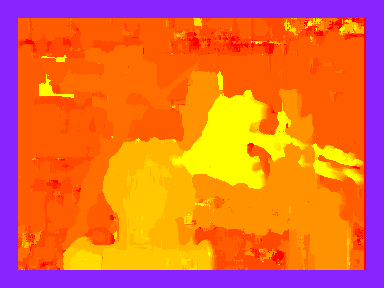
\includegraphics[width=0.45\textwidth]{src/images/evaluation/snsm-tsukuba-disparity-map.png}} \\
\subfloat[outliers in SNSM]{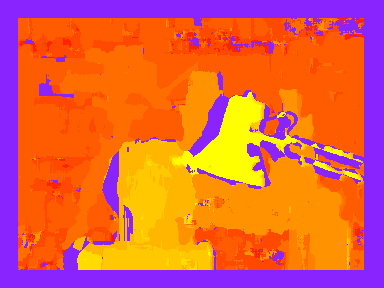
\includegraphics[width=0.45\textwidth]{src/images/evaluation/snsm-tsukuba-outliers.png}} &
\subfloat[outliers in SAD-IGMCT]{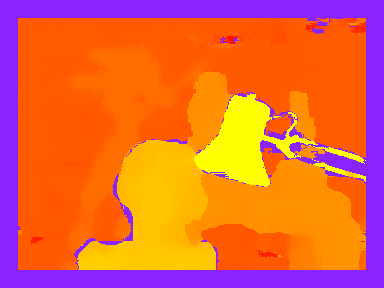
\includegraphics[width=0.45\textwidth]{src/images/evaluation/snsm-tsukuba-outliers-igmct.png}}
\end{tabular}
\caption{SNSM heatmaps for Tsukuba scene}
\label{fig:eval:snsm:tsukuba}
\end{figure}

\noindent In the beforehand mentioned Figure \ref{fig:eval:snsm:tsukuba}, SNSM struggles with the disparity constraints as they are not forced programmatically.
For each point $(x,y)$ the disparity is calculated individually.
This leads to a more noisy disparity map than for instance the disparity map of SAD-IGMCT, which respects the disparity constraints, takes the left-right-consistency into account and performs a disparity refinement step.
But it also shows that by implementing a simple stereo matcher with just the SAD as matching cost measurement step reasonable results can be achieved.
The semi-global stereo matcher implementation of OpenCV achieved the best result in PBMP$_{disc,2px}$, which focuses on the disparity estimation near depth-discontinuities at object borders.

\subsection{General performance}

From a theoretical perspective, the assumption is that the algorithms struggle with depth-discontinuity regions and arbitrary surfaces, i.e. textureless regions.
Also, global methods should perform slightly better than local methods.
Salient regions may a bit more random as they take the spectrum of the image into account and not the nature composition of pixel groups like textures.
As it would be a tremendous task to deliver all possible plots, only the highlights were included.
\newline\newline\noindent The following Tables \ref{fig:eval:general:performance1} and \ref{fig:eval:general:performance2} contain the general performance with the focus on PBMP$_{noc,1px}$.

\begin{table}[h!]
\centering
\scalebox{0.9}{
\begin{tabular}{c|rrrrrrrrr}
  & 1 & 2 & 3 & 4 & 5 & 6 & 7 & 8 & 9 \\ \hline
1 & 16.60\% & \cellcolor{red!50}30.98\% & 7.31\% & 19.55\% & 8.30\% & 8.74\% & 8.32\% & 24.35\% & \cellcolor{green!50}6.93\% \\
2 & \cellcolor{green!50}6.88\% & \cellcolor{red!50}13.90\% & 7.18\% & 30.75\% & 10.91\% & 11.19\% & 10.90\% & 13.10\% & 8.32\% \\
3 & 9.54\% & \cellcolor{red!50}28.14\% & 3.99\% & 11.18\% & 4.17\% & 4.25\% & 4.10\% & 6.31\% & \cellcolor{green!50}3.35\% \\
4 & 13.98\% & 18.86\% & 9.90\% & \cellcolor{red!50}23.53\% & 8.01\% & 10.47\% & \cellcolor{green!50}7.75\% & 10.20\% & 11.65\% \\
5 & 5.96\% & \cellcolor{red!50}16.13\% & \cellcolor{green!50}0.19\% & 1.37\% & 3.41\% & 3.34\% & 3.42\% & 5.68\% & 0.62\% \\ \hline
$\varnothing$ & 10,59\% & \cellcolor{red!50}21,60\% & \cellcolor{green!50}5,71\% & 17,28\% & 6,96\% & 7,60\% & 6,90\% & 11,93\% & 6,17\% 
\end{tabular}
}
\caption[Result table for general performance]{Result table for general performance, focusing on PBMP$_{noc,1px}$}
\label{fig:eval:general:performance1}
\end{table}

\noindent Focusing on the general performance of all but SNSM, ELAS outperforms in mean of all sequences the other global and local methods.
The worst result is achieved with the OpenCV block matching implementation.
It is also impressive that ELAS also outperforms traditional global methods, like graph cuts and belief propagation.
None the less, it has to be mentioned, that the performance of global methods may vary intensely depending on the formulation of the underlying energy function \citep{cyganek2011introduction, szeliski2008comparative, scharstein2006middlebury}.

\begin{table}[h!]
\centering
\scalebox{0.95}{
\begin{tabular}{c|rrrr}
  & 10 & 11 & 12 & 13 \\ \hline
1 & \cellcolor{red!50}32.61\% & \cellcolor{green!50}8.72\% & 10.07\% & 9.65\% \\
2 & \cellcolor{red!50}25.64\% & 11.79\% & \cellcolor{green!50}8.76\% & 8.90\% \\
3 & \cellcolor{red!50}13.26\% & \cellcolor{green!50}6.08\% & 8.71\% & 7.29\% \\
4 & \cellcolor{red!50}38.96\% & 12.98\% & \cellcolor{green!50}11.15\% & 11.26\% \\
5 & \cellcolor{red!50}8.60\% & \cellcolor{green!50}0.93\% & 4.54\% & 2.15\% \\ \hline
$\varnothing$ & \cellcolor{red!50}23,81\% & 8,10\% & 8,66\% & \cellcolor{green!50}7,85\% 
\end{tabular}
}
\caption[Result table for general performance]{Result table for general performance, focusing on PBMP$_{noc,1px}$}
\label{fig:eval:general:performance2}
\end{table}

\noindent It is interesting to see, that the simplest variant of the block matching implementation in OpenCV is outperformed by just a SAD matching cost implementation, the SNSM.
Also, the best results are achieved with the weighted spatiotemporal approach, although the approach was not superior in at least one sequence, but overall.

\subsubsection{Depth-discontinuity regions}

Figure \ref{fig:eval-plots-pbmp-disc1} depicts the trend of the percentage of bad matching pixels near depth-discontinuity areas.
It is clear to see that global methods perform better than local methods near object borders.
The worst results are achieved by simple block matching algorithms.
The best result is achieved by belief propagation, which tends to produce feasible results near object borders, also regarding other sequences.

\begin{figure}[h!]
\centering
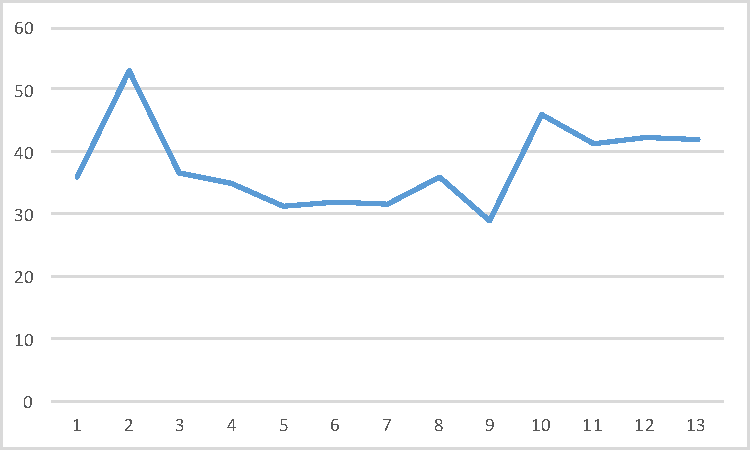
\includegraphics[width=1.0\textwidth]{src/images/evaluation/plots/01-book-pbmp-disc-1.pdf}
\caption[Chart of depth-discontinuity mask]{Depth-discontinuity mask applied on the book sequence with PBMP$_{disc,1px}$.}
\label{fig:eval-plots-pbmp-disc1}
\end{figure}

\noindent The graph shows also the correlation of the two metrics PBMP$_{disc,1px}$ and PBMP$_{noc,1px}$.
This means that each algorithm performs approximately the same way, either on depth-discontinuity areas or on non-occluded pixels with small positive displacement along the x-axis.
Concluding, the only algorithms which perform significantly worse than the others are the (2) OpenCV block matching implementation with filtering and (10) the simple OpenCV block matching implementation without filtering.
Although algorithm (4) MRF - ICM performs not as well as the others, it handles object borders at which depth-discontinuity occur more accurate than the other two outliers.
As this was just an example plot for depth-discontinuity areas, the other sequences behave the same way.

\subsubsection{Textureless regions}

\noindent The next Figure \ref{fig:eval-plots-pbmp-tex1} compares the amount of bad matching pixels in non-occluded regions with the textureless regions.
For this comparison, the tunnel scene of the Cambridge dataset was chosen.
It is clear to see that regions without textures, i.e. arbitrary surfaces are worse detectable than compared with textured objects.

\begin{figure}[h!]
\centering
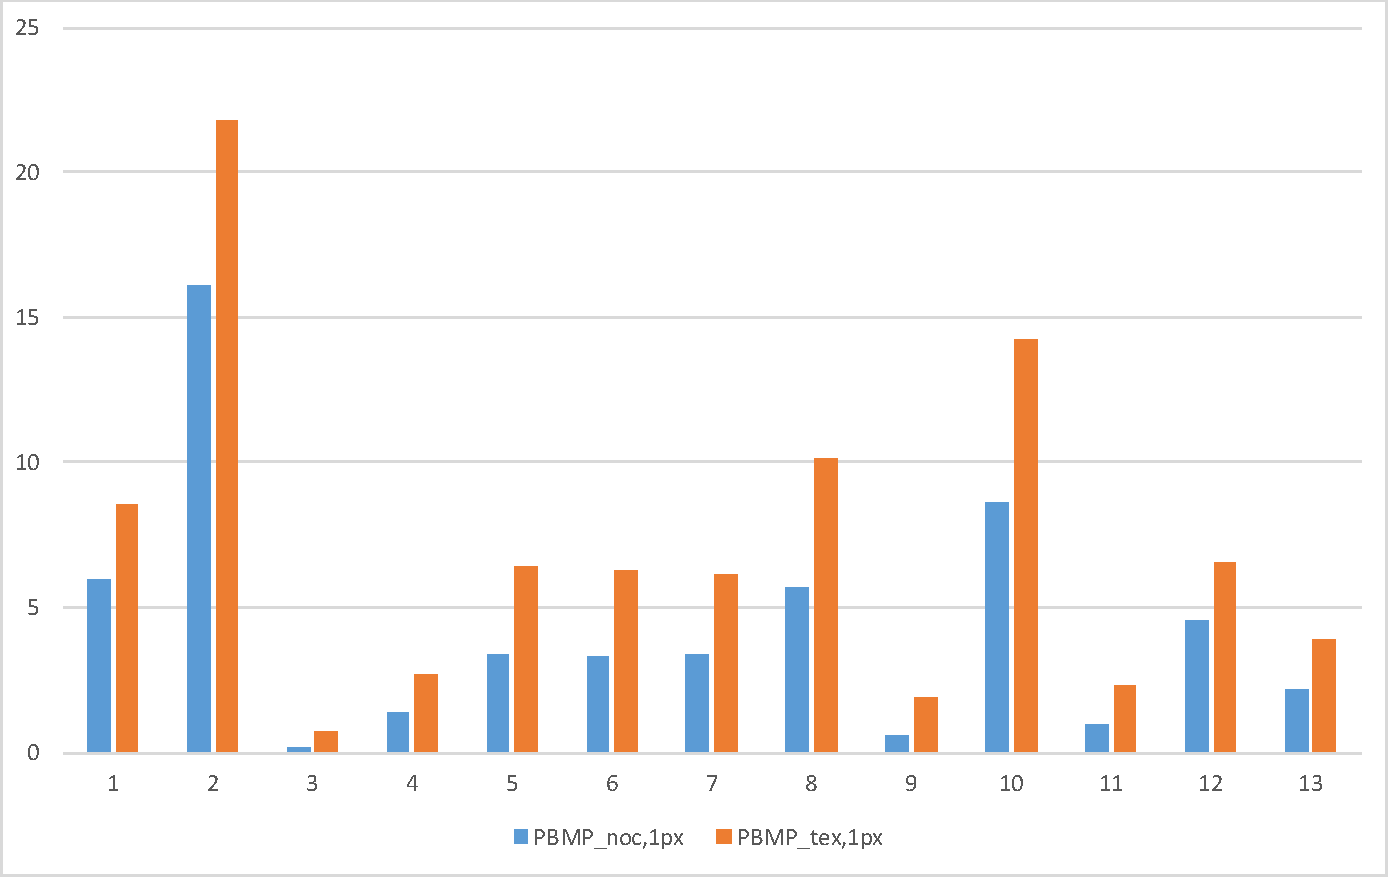
\includegraphics[width=1.0\textwidth]{src/images/evaluation/plots/05-tunnel-pbmp-tex-1.pdf}
\caption[Chart of textureless region mask]{Chart of textureless region mask applied on the tunnel sequence.}
\label{fig:eval-plots-pbmp-tex1}
\end{figure}

\noindent The percentage of bad matching pixels in textureless regions is nearly the same as overall in non-occluded areas, but with a positive displacement parallel to the x-axis.
It is also impressive that overall on average the ELAS algorithm yield to only 0.19\% of bad matching pixels in non-occluded regions PBMP$_{noc,1px}$.
In comparison, the worst algorithm, in this particular case the OpenCV block matcher implementation, resulted in PBMP$_{noc,1px}$ = 16.13\%.

\begin{table}[h!]
\centering
\scalebox{0.95}{
\begin{tabular}{l|rrrr}
  & RMSE$_{noc}$ & PBMP$_{noc,1px}$ & PBMP$_{noc,2px}$ & PBMP$_{noc,4px}$ \\ \hline
(3) ELAS & \cellcolor{green!50}0.36px & \cellcolor{green!50}0.19\% & \cellcolor{green!50}0.08\% & \cellcolor{green!50}0.04\% \\
(10) OpenCV - Simple BM & \cellcolor{red!50}5.82px & \cellcolor{red!50}8.60\% & \cellcolor{red!50}8.58\% & \cellcolor{red!50}8.56\% \\
(11) SNSM & 0.96px & 0.93\% & 0.71\% & 0.54\% \\
(12) SNSM STU & 1.02px & 4.53\% & 1.24\% & 0.73\% \\
(13) SNSM STW & 0.92px & 2.15\% & 0.79\% & 0.59\% \\
\hline
\end{tabular}
}
\caption[Result table for tunnel scene]{Result table for tunnel scene of Cambridge dataset}
\label{tab:eval:tex:tunnel:overview}
\end{table}

\noindent The SNSM also lead to feasible results which can be seen in Table \ref{tab:eval:tex:tunnel:overview}.
\newline\newline\noindent For a direct comparison of the visual outcome of the disparity maps, Figure \ref{fig:eval:heat:tunnel} depicts four images.
The left image with its ground-truth companion, the worst result of the OpenCV block matcher implementation and the best outcome yielded by ELAS.
ELAS seems to determine the disparity map in a nearly perfect manner but seems to struggle with the beginning shadow.

\begin{figure}[h!]
\centering
\begin{tabular}{cc}
\subfloat[left image]{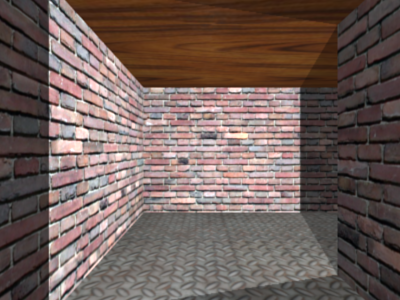
\includegraphics[width=0.45\textwidth]{src/images/evaluation/outliers2/tunnel-left.png}} &
\subfloat[ground-truth heatmap]{
\includegraphics[width=0.45\textwidth]{src/images/evaluation/outliers2/tunnel-ground-truth.png}} \\
\subfloat[outliers in OpenCV BM]{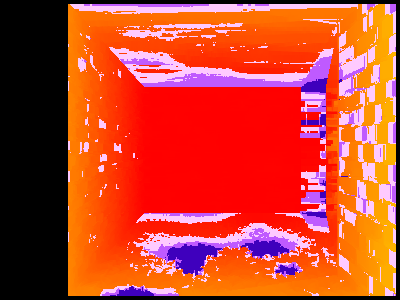
\includegraphics[width=0.45\textwidth]{src/images/evaluation/outliers2/tunnel-outliers-noc-2.png}} &
\subfloat[outliers in ELAS]{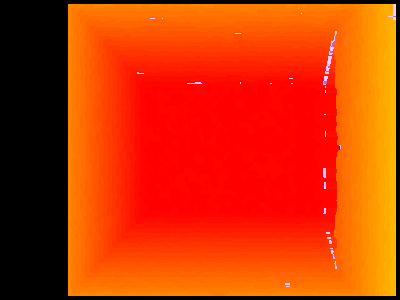
\includegraphics[width=0.45\textwidth]{src/images/evaluation/outliers2/tunnel-outliers-noc-3}}
\end{tabular}
\caption{Heatmaps for the tunnel scene}
\label{fig:eval:heat:tunnel}
\end{figure}

\noindent The SNSM led to feasible results in the tunnel scene, as can be seen in Table \ref{tab:eval:tex:tunnel:overview}.
The unweighted approach led to slightly worse overall results.
The interesting part here is the weighted approach of the SNSM implementation.
The RMSE$_{noc}$ improved whereas the PBMP$_{noc,1px}$ yield to shoddy results.
Considering both metrics, it shows that the naive spatiotemporal approach does not respect motion at all.
The slightly better RMSE$_{noc}$ feels a bit random in the overall evaluation.

\subsubsection{Salient regions}

Focusing on salient regions is a novel approach.
The distribution of salient regions does not follow any visual attracting regions.
According to \citeauthor{hou2007saliency} \citep{hou2007saliency}, the main idea is to extract the pixels which jump out of smooth curves, as they deserve most certainly the humans attention.
Their approach is implemented in the OpenCV library and no parameter can be set.
It is named static saliency, as only images are considered.
Thus, it is a pretty basic novel approach to create feasible masks with the static saliency.
The overall visual results are a bit confusing.
Figure \ref{fig:eval:sal:eg} shows two sample images and their corresponding computed saliency mask.
As can be seen in the figure, the static saliency approach in OpenCV yields to confusing results.
Although in both images, same parts, that are classified as salient regions, are comprehensible and understandable, some are not.

\begin{figure}[h!]
\centering
\begin{tabular}{cc}
\subfloat[image of book scene]{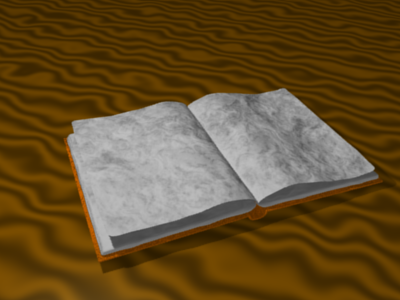
\includegraphics[width=0.45\textwidth]{src/images/evaluation/salient/left-book.png}} &
\subfloat[image of temple scene]{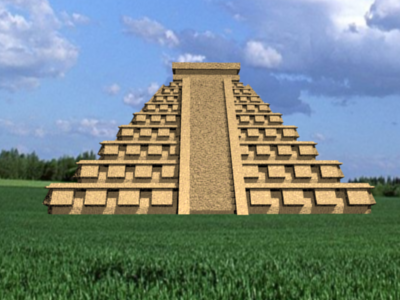
\includegraphics[width=0.45\textwidth]{src/images/evaluation/salient/left-temple.png}} \\
\subfloat[corresponding saliency mask]{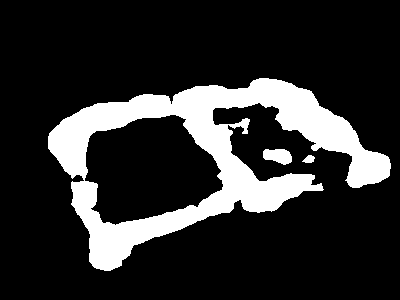
\includegraphics[width=0.45\textwidth]{src/images/evaluation/salient/salient-book.png}} &
\subfloat[corresponding saliency mask]{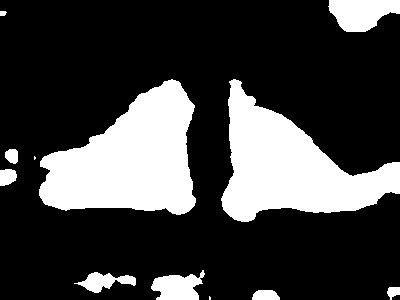
\includegraphics[width=0.45\textwidth]{src/images/evaluation/salient/salient-temple.png}}
\end{tabular}
\caption{Examples for salient masks}
\label{fig:eval:sal:eg}
\end{figure}

\noindent The book as a whole is not recognized as salient as well as the stairs of the temple are left out completely.
The chart in Figure \ref{fig:eval-plots-pbmp-sal} depicts the application of the saliency mask to the book sequence.

\begin{figure}[h!]
\centering
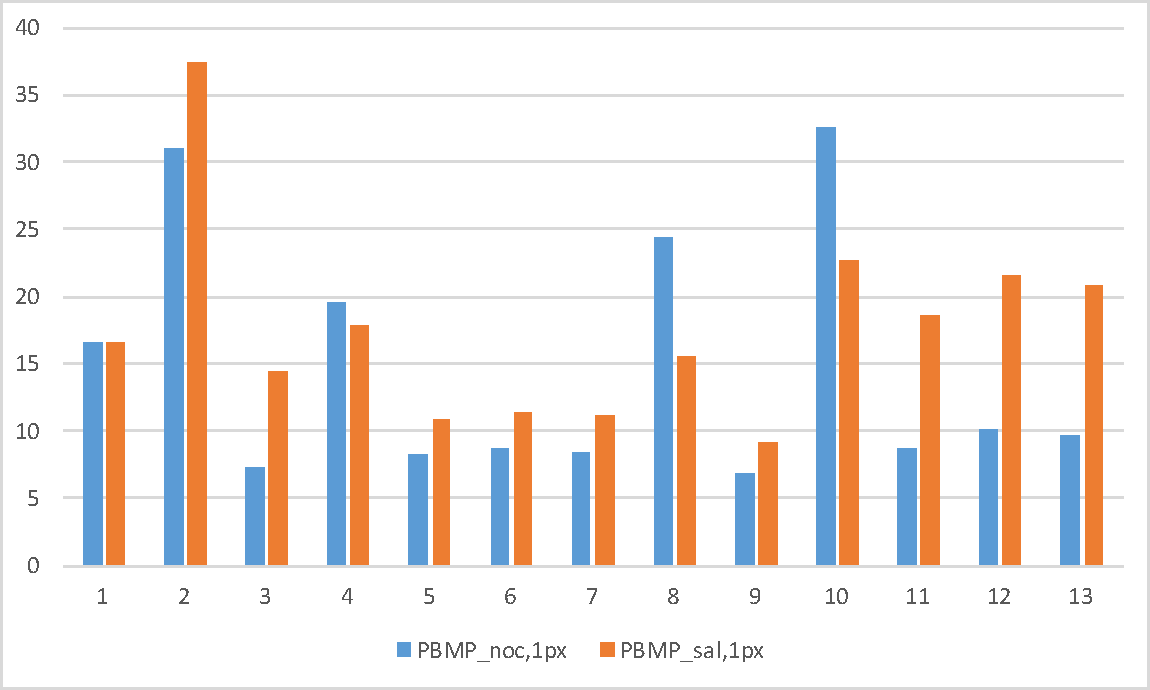
\includegraphics[width=1.0\textwidth]{src/images/evaluation/plots/01-book-pbmp-sal-1.pdf}
\caption[Chart of salient region mask]{Chart of salient region mask applied on the book sequence.}
\label{fig:eval-plots-pbmp-sal}
\end{figure}

\noindent The saliency mask has no real informative value.
There is no clear correlation identifiable.
In some cases, the saliency mask covers also depth-discontinuity areas and occluded areas.
Thus, it can yield to worse results than PBMP$_{noc,1px}$.
In other scenes of the Cambridge dataset, the results were similar to the book sequence.
Within high-resolution images, like the SVDDD dataset, the saliency mask looked even more unpredictable.
No clear salient regions were identifiable.
The assumption is that the algorithm, which is implemented in the OpenCV library is may be not capable of high-resolution images.
None the less, it could be shown, that the evaluation does not benefit from such a saliency mask.

\subsubsection{Outliers}

Beforehand, the investigation of outliers in a whole sequence of consecutive frames was mentioned.
During the evaluation, each sequence tended to have outliers.
To give an example, the book scene in combination with the (3) ELAS algorithm was chosen.
In this scene, two frames have significant more bad matched pixels than all the others, $23$ and $26$ although the margin is low.
The scenes shows a book.
During 41 frames one page will be turned over.

\begin{figure}[h!]
\centering
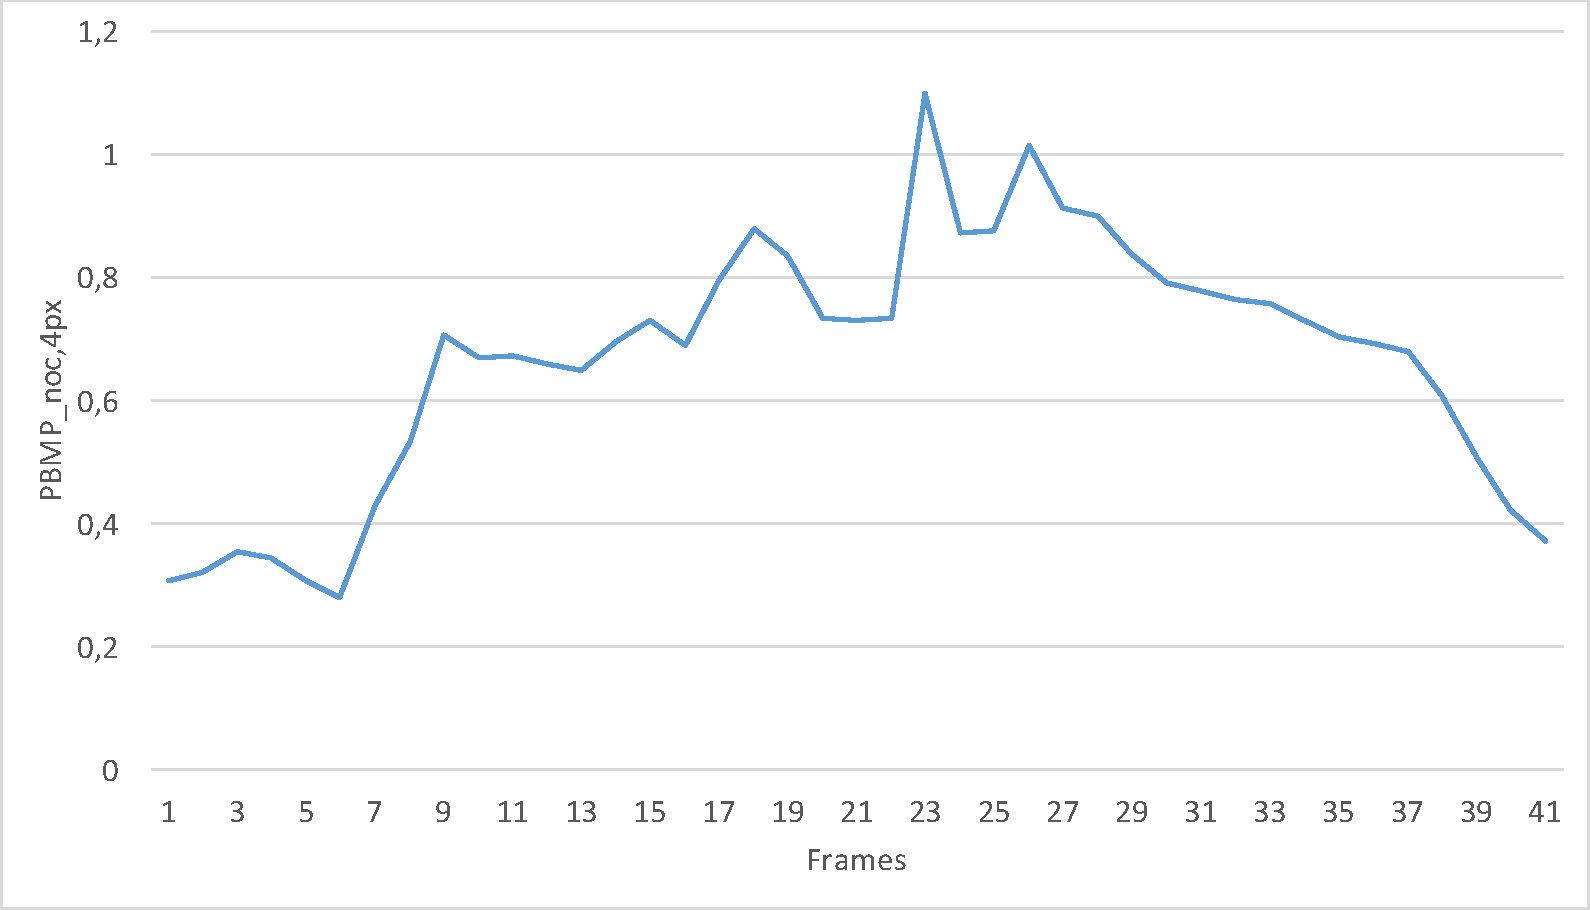
\includegraphics[width=1.0\textwidth]{src/images/evaluation/plots/01-book-general-outliers.pdf}
\caption[Chart of general outliers in a sequence]{Chart of general outliers in a sequence.}
\label{fig:eval-plots-outliers}
\end{figure}

\noindent The Figure \ref{fig:eval-plots-outliers} shows that in the beginning and in the end of the scene, exactly the point, in which the page is turned over and forms a flat surface with the book.
During the movement of the page, more object borders are created as the thin page forms a new object.
In frame $23$ and $26$ the turn over from one side to the other is made.
Thus, in exactly this two frames the amount of depth-discontinuity borders is the highest.
Figure \ref{fig:eval:out:eg} depicts these frames.
The increasing error at those object borders can be identified.
It is also clearly visible that Frame $23$ has the highest percentage  of bad matching pixels.

\begin{figure}[h!]
\centering
\begin{tabular}{ccc}
\subfloat[Frame 1]{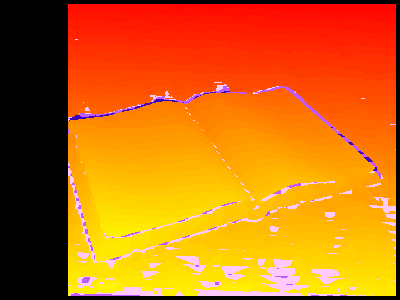
\includegraphics[width=0.3\textwidth]{src/images/evaluation/outliers/image0001.png}} &
\subfloat[Frame 23]{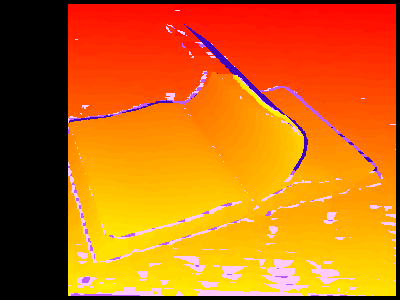
\includegraphics[width=0.3\textwidth]{src/images/evaluation/outliers/image0023.png}} &
\subfloat[Frame 26]{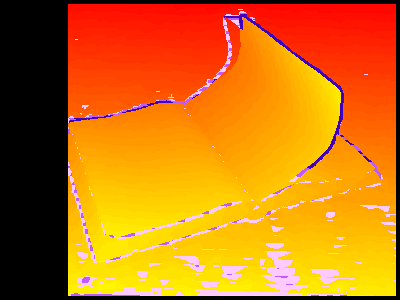
\includegraphics[width=0.3\textwidth]{src/images/evaluation/outliers/image0026.png}} \\
\end{tabular}
\caption[Examples for general outliers in a sequence]{Examples for general outliers in the book sequence. The disparity maps are computed with the (3) ELAS algorithm.}
\label{fig:eval:out:eg}
\end{figure}

\subsection{Impact of noise}

The impact of noise is an interesting and not often evaluated approach regarding disparity algorithms.
For this observation five different datasets were created with the image diminisher.
The Cambridge dataset was cloned and each image in this dataset was diminished with a newly created noise mask.
The noise mask was added on top of the image matrix.
Different values were chosen as mentioned in the measurement section.
For demonstration purpose, a plot, which contains all three $sigma^2$ values was chosen.
Figure \ref{fig:eval-plots-gn-overview} shows the impact of different $\sigma^2$ values for additive Gaussian noise on the computation of disparity algorithms.

\begin{figure}[h!]
\centering
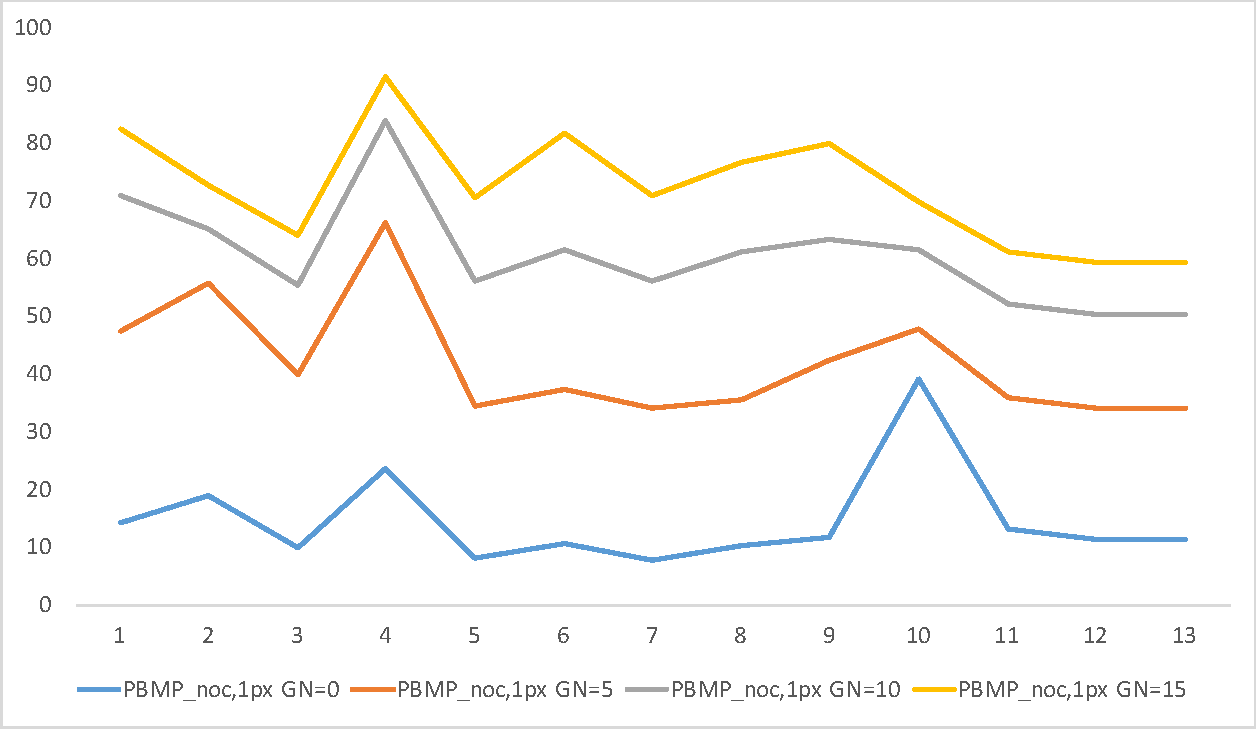
\includegraphics[width=1.0\textwidth]{src/images/evaluation/plots/04-temple-gn-overview.pdf}
\caption[Chart of the impact of Gaussian noise]{Chart of the impact of different $\sigma^2$ values for additive Gaussian noise on the result of disparity algorithms focusing on P$_{noc,1px}$.}
\label{fig:eval-plots-gn-overview}
\end{figure}

\noindent Here, the tunnel scene was picked to demonstrate the impact of normal distributed noise.
Although, as mentioned beforehand in Chapter \ref{chap:impl}, the idea follows the methodology of \citeauthor{richardt2010real} \citep{richardt2010real}, it is not clear if additive Gaussian noise is an adequate image diminishing effect to simulate real scenery.
None the less, it is nice to see that all picked metrics correlate with each other.
The extent of the displacement along the x-axis depends on the amount of disturbing noise was added.
Figure \ref{fig:eval:gn:eg} depicts the first frame of the tunnel sequence with different noise degrees.
Added noise with a $sigma^2$ of $5$ does not seem to distract the visual appearance of the image.
None the less, it has a direct impact on the performance of disparity algorithms.
The degree of noise with a $\sigma^2$ of $15$ is visually noticeable.
One reason for that might be, that this type of noise may not appear in real-life while capturing a scene with a CCD sensor.
The approach follows the methodology of \citeauthor{richardt2010real} \citep{richardt2010real} but may not be suitable for simulating real scenery.
But, for the purpose of simulating an image, captured via CCD sensor, camera noise models exist \citep{liu2006noise}.
The approach with additive Gaussian noise changes every pixel in the image, by a different amount.
But an image, captured via CCD sensor, does not seem to have this pattern (cf. \citep{liu2006noise}).
Changing every pixel, even by a small amount means that the calculated matching cost may differ largely.
This is of course depending on other factors, such as window size and which matching cost formula is applied.
The assumption remains, that additive Gaussian noise may not be a good choice to simulate real scenery and to measure the in uence on disparity algorithms.

\begin{figure}[h!]
\centering
\begin{tabular}{cc}
\subfloat[temple frame]{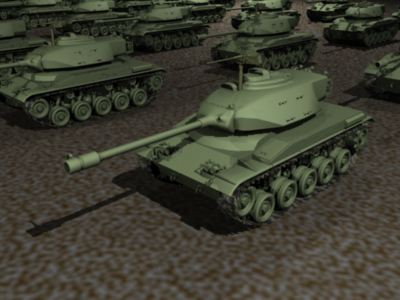
\includegraphics[width=0.45\textwidth]{src/images/evaluation/outliers-gn/image0001.png}} &
\subfloat[$\sigma^2=5$]{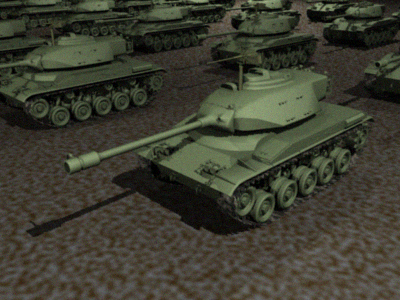
\includegraphics[width=0.45\textwidth]{src/images/evaluation/outliers-gn/image0001-gn5.png}} \\
\subfloat[$\sigma^2=10$]{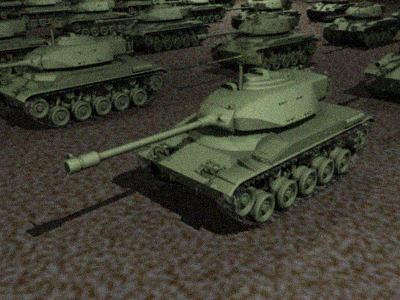
\includegraphics[width=0.45\textwidth]{src/images/evaluation/outliers-gn/image0001-gn10.png}} &
\subfloat[$\sigma^2=15$]{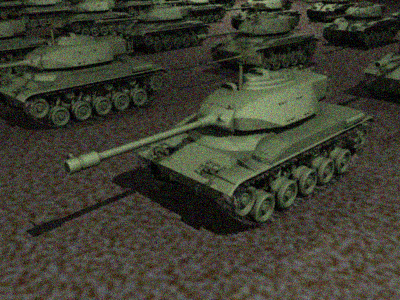
\includegraphics[width=0.45\textwidth]{src/images/evaluation/outliers-gn/image0001-gn15.png}}
\end{tabular}
\caption{Examples for image diminishing effects with Gaussian noise}
\label{fig:eval:gn:eg}
\end{figure}

\noindent The upcoming subsection also deals with image diminishing effects, in this case video compression.

\subsection{Impact of video compression}

The impact of video compression is an interesting and novel approach.
High-resolution videos, due to its nature, are not shipped for television as uncompressed raw data or even lossless compressed.
As seen in the Chapter \ref{chap:related}, there are different applications for disparity algorithms.
One outpointed need is the remapping of disparity for different screen sizes.
If this can not happen on raw data, for instance the data is missing and only the compressed version is available, the influence of video compression on the outcome of disparity algorithms is observed.
\noindent For this observation five different datasets were created with the image diminisher.
As underlying video codec H.265 was chosen because it is currently the most efficient video compression technique.
The recommended default parameter for H.265, the constant rate factor (CRF) is $28$.
It ranges from $0-51$, whereas $0$ represents lossless and $51$ the worst possible compression.
$0, 14, 28, 40, 51$ were chosen with $14$ and $40$ as additionally in-between parameters.
$0$ and $51$ were left out, as the result is too visually distracting for the viewer with $51$ and $0$ is lossless.
Thus, the observed values are $14, 28, 40$.

\begin{figure}[h!]
\centering
\begin{tabular}{ccc}
\subfloat[book, CRF = 14]{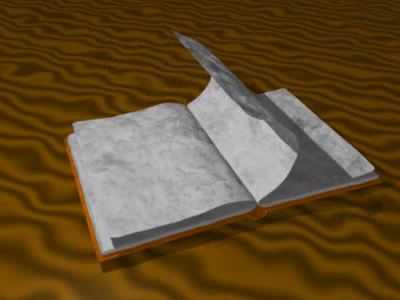
\includegraphics[width=0.3\textwidth]{src/images/evaluation/outliers-vc/book-image0022-vc14.png}} &
\subfloat[book, CRF = 28]{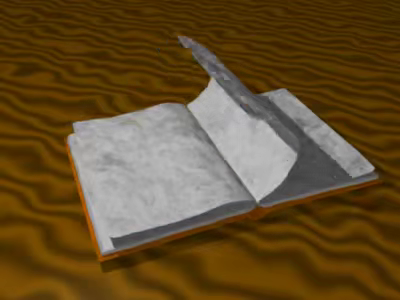
\includegraphics[width=0.3\textwidth]{src/images/evaluation/outliers-vc/book-image0022-vc28.png}} &
\subfloat[book, CRF = 40]{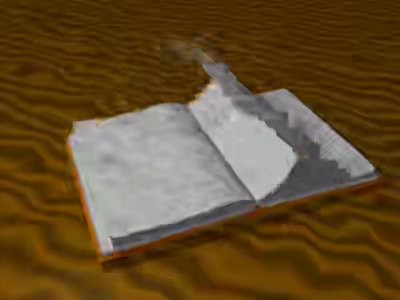
\includegraphics[width=0.3\textwidth]{src/images/evaluation/outliers-vc/book-image0022-vc40.png}} \\
\subfloat[tanks, CRF = 14]{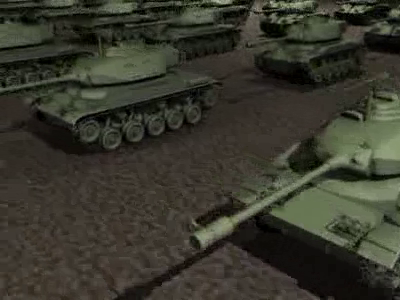
\includegraphics[width=0.3\textwidth]{src/images/evaluation/outliers-vc/tanks-image0023-vc14.png}} &
\subfloat[tanks, CRF = 28]{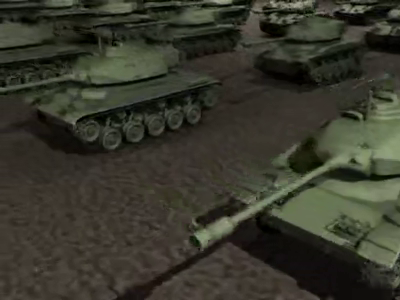
\includegraphics[width=0.3\textwidth]{src/images/evaluation/outliers-vc/tanks-image0023-vc28.png}} &
\subfloat[tanks, CRF = 40]{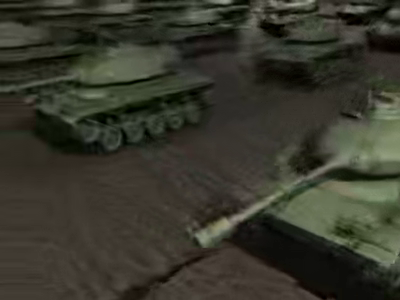
\includegraphics[width=0.3\textwidth]{src/images/evaluation/outliers-vc/tanks-image0023-vc40.png}} \\
\end{tabular}
\caption[Examples for image diminishing effects with video compression]{Examples for image diminishing effects caused by video compression artifacts of the H.265 codec in combination with different values for CRF.}
\label{fig:eval:vc:eg}
\end{figure}

\noindent Figure \ref{fig:eval:vc:eg} depicts the effect of different CRF values using H.265.
It is clearly visible that a CRF with $14$ leads to feasible results regarding the experience for viewers.
A CRF with $28$ and $40$ lead to more distracting artifacts.
Figure \ref{fig:eval-plots-pbmp-noc1-vc} illustrates the correlation of the H.265 CRF and PBMP$_{noc,1px}$.
Even the lowest value in test series, $14$ leads to a huge amount of bad matching pixels.
A CRF with $28$ seems to as hard as $14$ for disparity algorithm, as the amount of bad matching pixels is nearly identical with the amount of $14$.

\begin{figure}[h!]
\centering
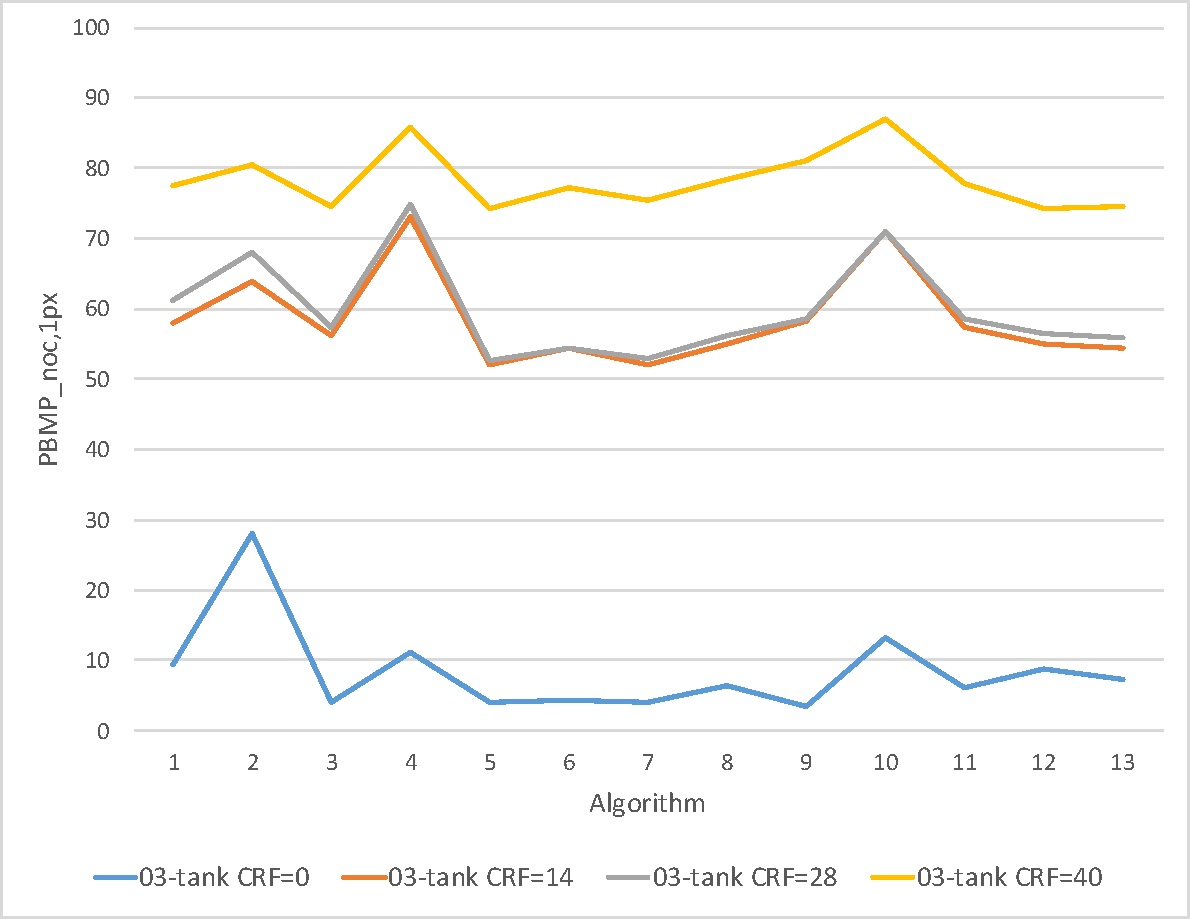
\includegraphics[width=1.0\textwidth]{src/images/evaluation/plots/03-tank-pbmp-noc-1-vc.pdf}
\caption[Chart of the impact of video compression]{Chart of the impact of different CRF values for H.265 video compression on the result of disparity algorithms focusing on PBMP$_{noc,1px}$.}
\label{fig:eval-plots-pbmp-noc1-vc}
\end{figure}

\noindent Figure \ref{fig:eval:vc:eg2} depicts the computed disparity maps after diminishing the whole scene with a CRF value of $40$.
Many disparity information seem to be lost.
The structure of the fire pipe of the right tank is still visible and the disparity information are valid within a threshold of $1px$.
The rest feels a bit random.
\newline\newline\noindent Talking about SNSM, it lead to better results than most of the other algorithms.
In the tank sequence, (11) SNSM achieved PBMP$_{noc,1px}$ = 80.72\% where as (8) MRF - BP BPM achieved 82.45\%, which led to superior results beforehand.
The unweighted and weighted approach were able to improve this result to 75.04\% and respectively 75.58\%.

\begin{figure}[h!]
\centering
\begin{tabular}{ccc}
\subfloat[(3) ELAS outliers]{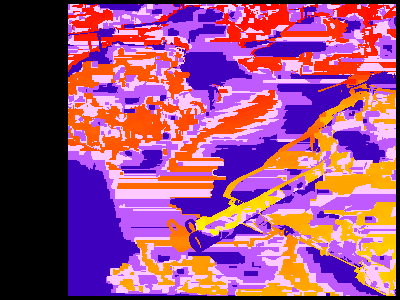
\includegraphics[width=0.3\textwidth]{src/images/evaluation/outliers-vc/image0023-heatmap-outliers-3.png}} &
\subfloat[(5) MRF GC Swap outliers]{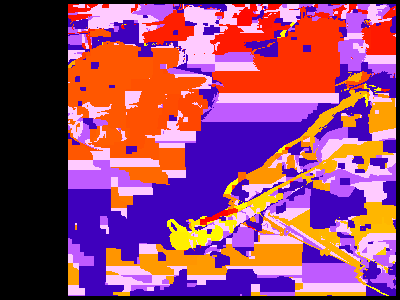
\includegraphics[width=0.3\textwidth]{src/images/evaluation/outliers-vc/image0023-heatmap-outliers-5.png}} &
\subfloat[(13) SNSM STW]{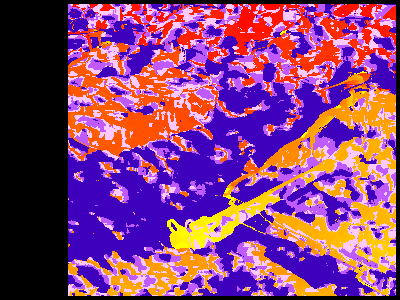
\includegraphics[width=0.3\textwidth]{src/images/evaluation/outliers-vc/image0023-heatmap-outliers-13.png}} \\
\end{tabular}
\caption[Example of computed disparity maps with video compression]{Example of computed disparity maps with video compression. CRF is set to $40$. Frame 23 of the tanks scene.}
\label{fig:eval:vc:eg2}
\end{figure}

\subsection{Runtime}

Talking about runtime, the results differ vastly.
Figure \ref{fig:eval-plots-runtime} illustrates the different runtimes in mean over all sequences of the Cambridge dataset.
This should provide a solid overview.
It is clear to see that four variants run fast, i.e. have a low runtime.
This is true for the local methods, as well as ELAS.
The global methods need much more time to approximate the energy function.
\newline\newline\noindent Especially the algorithm variants of belief propagation needed much time.
Throughout the whole evaluation, (8) MRF - BP BPM led to the best results, compared with other global methods.
The runtime is according to algorithm (7) MRF - BP TRWS and (9) MRF - BP BPM the lowest.
Comparing with other results, which were outlined in the sections before, the runtime is not justified as the longer an algorithm runs does not automatically yield to better results.
\newline\newline\noindent The (11) SNSM is the worst local method focusing on the runtime in comparison with (1), (2) and (10), which are all OpenCV implementations of block matching algorithms.
This may result as the whole disparity space image is calculated beforehand the disparity maps are computed.
So the runtime of the SNSM is basically the runtime for the whole scene divided through the amount of frames.
Both variants, the (12) SNSM-STU and (13) SNSM-STW are dealing with the same information in the same way besides the assembly of the matching cost.
But this should not affect the runtime at all, so it is also clearly to see, that a certain deviation of the runtime has to be kept in mind.
\newline\newline\noindent ELAS outperformed in many times all the other algorithms according to PBMP$_{noc}$.
The runtime is feasible for real-time applications but slightly worse than simple local methods, like the OpenCV block matcher implementation.
Although, it has to be kept in mind, as outlined in Chapter \ref{chap:impl}, that ELAS is a library which comes with a front-end and an internal image library.
Both can be the origin for the runtime being worse than simple block-matching algorithm.
For an accurate comparison which approach is faster, both should be implemented utilizing the same underlying image library.

\begin{figure}[h!]
\centering
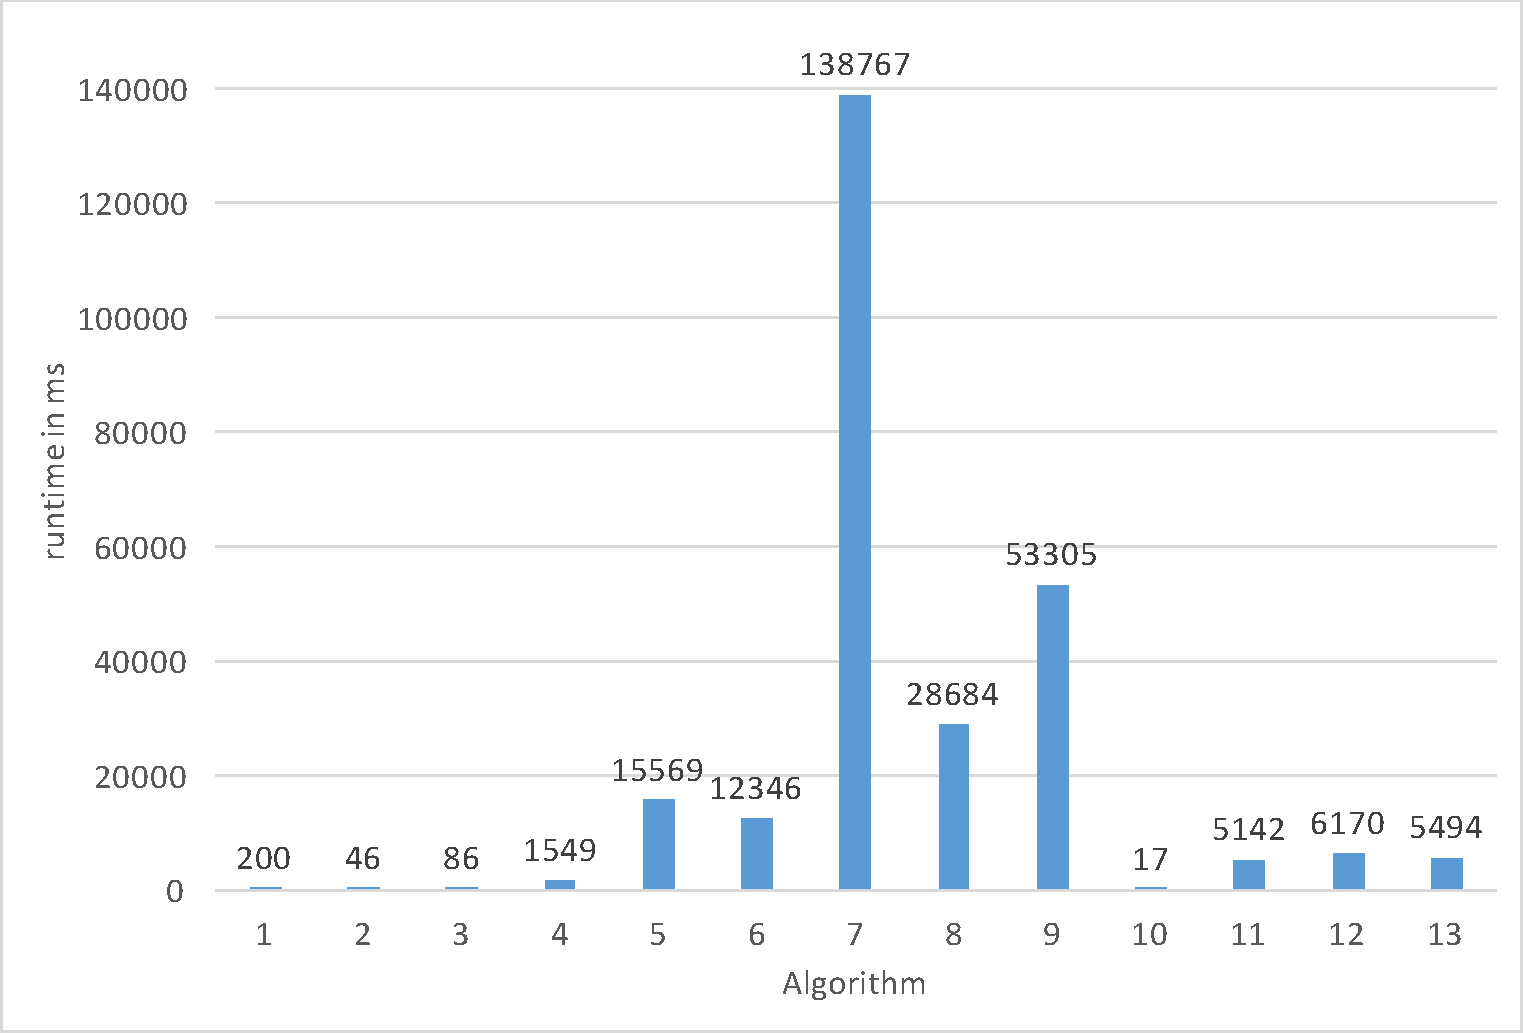
\includegraphics[width=1.0\textwidth]{src/images/evaluation/plots/runtime.pdf}
\caption[Comparison of the runtime of different disparity algorithms]{Comparison of the runtime of different disparity algorithms}
\label{fig:eval-plots-runtime}
\end{figure}

\subsection{SVDDD}

The SVDDD dataset from the department of Praktische Informatik IV\footnote{\url{http://ls.fmi.uni-mannheim.de/de/pi4/}} was evaluated as well.
During this thesis, the dataset ran through several iterations as more and more problems arose during the evaluation.
In addition, some algorithms were not able to process high-resolution stereo images.
Thus, it is separated from the other results.
\newline\newline\noindent The initially evaluated scenes led to strange results.
Some areas were computed correctly but some areas were completely off.
One major point, which can lead to such strange, defective results, is negative disparity.
Most of the algorithms expect that disparity values range from $0-d_{max}$.
Even a small amount of negative disparity can conduct to a result, which is slightly off, i.e. three or four pixels.
Looking at PBMP$_{1px}$ , which can yield to nearly $50\%$.
An example can be seen in Figure \ref{fig:outliers-rabbit-svddd}, illustrating two images.
In the left image about $10\%$ pixels overall contains slightly negative disparity whereas in the right image, the disparity ranges from $0-59$.

\begin{figure}[h!]
\centering
\begin{tabular}{ccc}
\subfloat[Negative disparity]{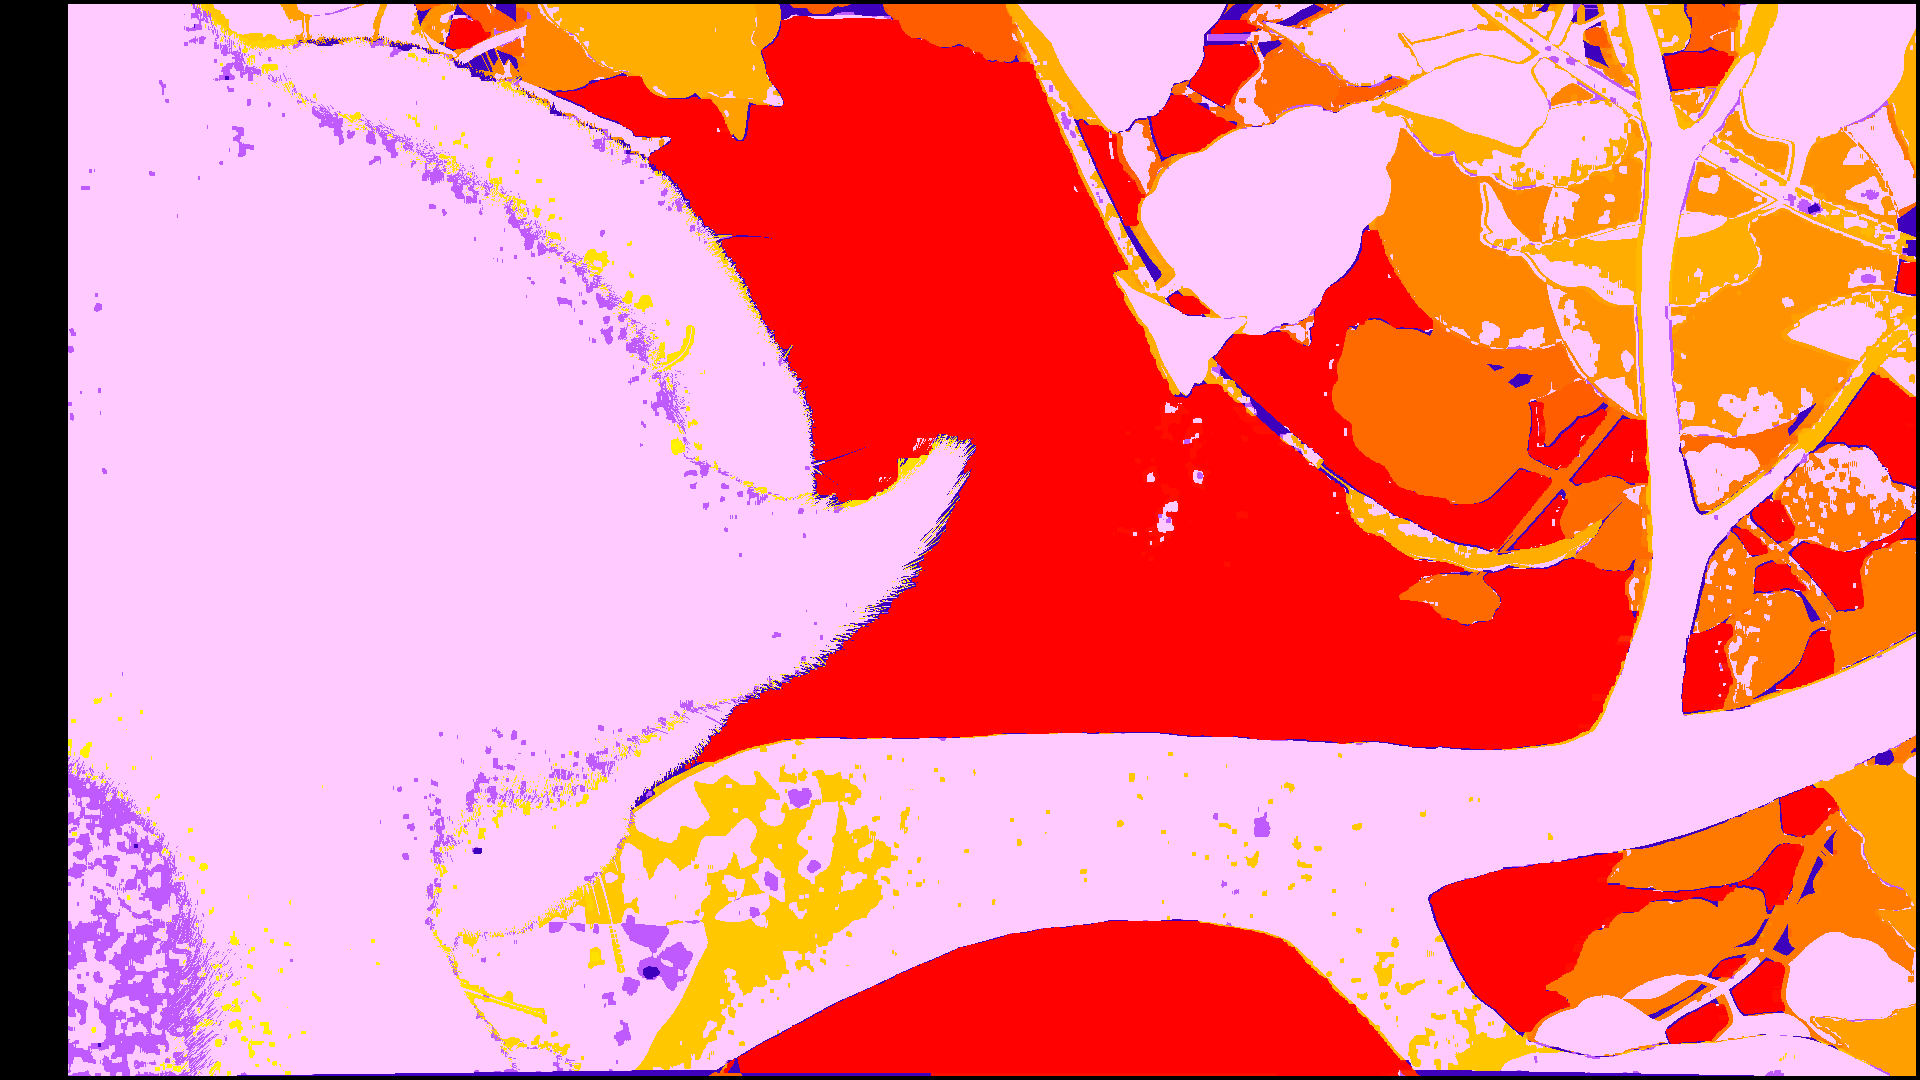
\includegraphics[width=0.48\textwidth]{src/images/evaluation/02-rabbit-neg-elas.png}} &
\subfloat[Only positive disparity]{\includegraphics[width=0.48\textwidth]{src/images/evaluation/02-rabbit-elas.png}} &
\end{tabular}
\caption[Computed disparity map with negative disparity]{Comparison of computed disparity maps regarding negative disparity.}
\label{fig:outliers-rabbit-svddd}
\end{figure}

\noindent Another challenge of high-resolution datasets is the huge computational power, which is necessary to compute disparity maps for them.
The BP algorithms would have needed about $52 GB$ of memory to calculate the scenes for $d_{max} = 64$ as the labels for all possible states have to be created and stored in memory.
Also, the SNSM wanted to allocate about $35 GB$ of memory as the disparity space image is computed \textit{a priori} before the actual calculation of the disparity maps takes place.
The runtime also gives a feeling how computational powerful and complex it is, to perform a disparity estimation on high-resolution stereo images.
Summing up, the MRF BP algorithms as well as the SNSM were excluded from the evaluation of the SVDDD dataset.

\begin{table}[h!]
\centering
\scalebox{1.0}{
\begin{tabular}{l|rrrrrr}
  & 1 & 2 & 3 & 4 & 5 & 6 \\ \hline
02-rabbit-neg & 58.62\% & \cellcolor{red!50}61.51\% & 59.99\% & 60.58\% & \cellcolor{green!50}57.12\% & 57.13\% \\
02-rabbit & 1.68\% & \cellcolor{red!50}4.31\% & 2.98\% & 3.82\% & \cellcolor{green!50}0.65\% & 0.68\% \\
03-apple & 1.69\% & \cellcolor{red!50}4.10\% & 3.11\% & 3.44\% & \cellcolor{green!50}0.63\% & 0.65\% \\ \hline
$\varnothing$ (w/o neg) & 1.69\% & \cellcolor{red!50}4.21\% & 3.05\% & 3.63\% & \cellcolor{green!50}0.64\% & 0.67\%
\end{tabular}
}
\caption[Result table for general performance of SVDDD]{Result table for general performance of SVDDD, focusing on PBMP$_{noc,1px}$}
\label{tab:svddd-performance}
\end{table}

\noindent Table \ref{tab:svddd-performance} contains the mean results of the SVDDD dataset.
The best result is achieved with the MRF GC Expansion algorithm, which only led to $0.64\%$ of bad matching pixels in all scenes which is quite impressive for both, the scenes and the algorithms.
OpenCV SGBM and ELAS also lead to good results.
Comparing the runtime of such high-resolution scenes, the (2) OpenCV BM clearly outperforms the others.
Taking the general performance into account, OpenCV SGBM and ELAS both yield to feasible results.
For real-time applications ELAS stands out against the other algorithms.
Taking both, the overall performance and the runtime into account, ELAS performs best.
In Figures \ref{fig:eval-svddd-plot-rabbit} and \ref{fig:eval-svddd-plot-apple}, it is clearly to see that ELAS also performs better than the other local methods regarding PBMP$_{noc,4px}$.

\begin{figure}[h!]
\centering
\includegraphics[width=1.0\textwidth]{src/images/evaluation/svddd/02-rabbit-plot.pdf}
\caption[Performance of SVDDD rabbit scene]{Performance of SVDDD rabbit scene}
\label{fig:eval-svddd-plot-rabbit}
\end{figure}

\noindent Both scenes, rabbit and apple performed pretty reasonable.
In direct comparison with the Cambridge datasets, the results are better.
The Cambridge scenes are unrealistic constructed in comparison to the Big Buck Bunny project as they contain a lot of repeating objects and arbitrary textures.
Even the tunnel scenery contains many identical looking bricks.
The literature states, that those textures are error-prone areas, this could be a reason for the better performing SVDDD.
The coloring of the scenes in the Cambridge dataset is very even distributed whereas the SVDDD dataset contains different colors in each scene.
Some scenes of the Cambridge dataset led to worse result than the others, especially the street scene performed best, which supports the assumption, that the result rely on the composition of the scenery.
In the beginning, the assumption arose, that the fine hair textures may be problematic.
This is not the case.
The computed disparity map lack of accuracy near depth-discontinuity areas, but fine-grained structures were not problematic at all.

\begin{figure}[h!]
\centering
\includegraphics[width=1.0\textwidth]{src/images/evaluation/svddd/03-apple-plot.pdf}
\caption[Performance of SVDDD apple scene]{Performance of SVDDD apple scene}
\label{fig:eval-svddd-plot-apple}
\end{figure}

\noindent Focusing on the runtime, which is illustrated in Table \ref{tab:svddd-runtime}, the fastest algorithm is again the OpenCV BM implementation.
But the huge gap between (2) ELAS, (3) OpenCV BM and the others is noticeable.
ELAS seems to be a pretty solid approach regarding runtime and overall performance of disparity estimation.
The best results were achieved by the global methods, which pretty astonishing results of PBMP$_{noc,1px} < 1\%$.
The runtime was very bad with nearly 10 minutes to compute one single disparity map.
It has to be kept in mind, that the computation depends heavily on the underlying computing engine (CPU or GPU) and also the implementation.
Also, in difference to the Cambridge dataset, the SVDDD dataset led to endless iterations in the Middlebury library.
The Middlebury library is kept to a maximum of 500 iterations, which is not adjustable.
The SVDDD dataset always needed the whole iterations, which may be the reason for such a long runtime.
A reason for that can be the high resolution of the dataset.

\begin{table}[h!]
\centering
\scalebox{0.9}{
\begin{tabular}{l|rrrrrr}
  & 1 & 2 & 3 & 4 & 5 & 6 \\ \hline
02-rabbit-neg & 6550 ms & \cellcolor{green!50}817 ms & 1923 ms & 11796 ms & 300939 ms & \cellcolor{red!50}544833 ms \\
02-rabbit & 4402 ms & \cellcolor{green!50}465 ms & 1000 ms & 20141 ms & 420835 ms & \cellcolor{red!50}617998 ms \\
03-apple & 4541 ms & \cellcolor{green!50}467 ms & 984 ms & 16063 ms & 384221 ms & \cellcolor{red!50}575137 ms \\ \hline
$\varnothing$ & 5164 ms & \cellcolor{green!50}583 ms & 1302 ms & 16000 ms & 368665 ms & \cellcolor{red!50}579323 ms
\end{tabular}
}
\caption[Result table for runtime of SVDDD]{Result table for runtime of SVDDD}
\label{tab:svddd-runtime}
\end{table}

\section{Discussion}

In this section, the result seen before are summarized and discussed.
The general performance of the integrated algorithms in comparison with the simple naive stereo matcher (SNSM) is interesting.
The outcome of the comparison is, that in general local methods are faster than global methods but the quality benefit of the disparity map may not be high.
Although, this depends heavily on the use-case, only one global method, the (9) MRF - BP BPM was really superior.
SNSM is on a level playing field with other global methods, and even outperforms some, like (3) MRF ICM and (8) MRF - BP BPS.
Taking the spatiotemporal context into account yields overall to better results, but still lacks of respecting the motion of objects.
Thus, the result may be a bit random regarding this particular case, as mentioned beforehand in Chapter \ref{chap:impl}.
The masks are granting another perspective on the performance of disparity algorithms, but only the depth-discontinuity as well as the non-occluded pixel mask seem to give a real overall benefit.
The saliency mask seems to bit more random as most of the salient regions are not marked correctly whereupon the room for interpretation when it comes to saliency has to be kept in mind.
\newline\newline\noindent The results regarding Gaussian noise differ from the results, which \citeauthor{richardt2010real} \citep{richardt2010real} achieved.
Here, a much lower $\sigma^2$ led to defective results.
As every pixel gets changed according to the normal distribution and additionally, for each image a different noise matrix was calculated to avoid pattern matching, the stereo image gets disturbed in an unnatural way.
\citeauthor{richardt2010real} added additive Gaussian noise to simulate a more natural, real scenery.
Gaussian noise is a part of sensor noise, but a small one.
To simulate such real scenery, a more realistic model should be created.
For the purpose of simulating an image, captured via CCD sensor, camera noise models exist \citep{liu2006noise}.
Such complex noise models are difficult to create, but maybe lead to much more feasible results.
Here, it could be shown that a small amount of normal distributed noise lead to false disparity information.
The small amount of informative value is may be at random computed.
\newline\newline\noindent With testing the interference of video compression, a novel approach was shown.
The outcome of the approach is, that even a small amount of video compression artifacts lead to a lot of mismatched pixels, although the artifacts are not clearly visible.
As two parameters are correlating directly and the change of the CRF from $14$ to $28$ did not change the overall result, it may be the case, that disparity algorithms struggle with a small amount of noise until a certain level.
The jump from about 10\% of bad matching pixels to nearly 60\% at the first tested step is huge.
\newline\newline\noindent Taking the runtime into account, the information taken out of the literature were confirmed.
Global methods tend to run pretty long whereas local methods are more for real-time applications.
Here, ELAS established itself as a surprise candidate.
The overall performance combined with the runtime is good.
The results towards object borders are accurate.
Depending on the image resolution, global methods struggle with high-resolution images whereas ELAS performed pretty well.
\newline\newline\noindent The last part of the evaluation was to benchmark the SVDDD dataset of the department of Praktische Informatik IV\footnote{\url{http://ls.fmi.uni-mannheim.de/de/pi4/}}.
After initial problems with the range of disparity values as well as some ground-truth disparity maps contained unfeasible values, two final scenes could be evaluated.
Both scenes performed very good along all algorithms.
Here, the computational limitations became noticeable as the belief propagations as well as the SNSM implementation were in need of too much memory.
None the less, the other algorithms drew the bigger picture with the main outcome, that the OpenCV SGBM implementation as well as ELAS performed best.
